%% Le lingue utilizzate, che verranno passate come opzioni al pacchetto babel. Come sempre, l'ultima indicata sar� quella primaria.
%% Se si utilizzano una o pi� lingue diverse da "italian" o "english", leggere le istruzioni in fondo.
\def\thudbabelopt{english}
%% Valori ammessi per target: bach (tesi triennale), mst (tesi magistrale), phd (tesi di dottorato).
%% Valori ammessi per aauheader: '' (vuoto -> nessun header Alpen Adria Univeristat), aics (Department of Artificial Intelligence and Cybersecurity), informatics (Department of Informatics Systems). Il nome del dipartimento � allineato con la versione inglese del logo UniUD.
%% Valori ammessi per style: '' (vuoto -> stile moderno), old (stile tradizionale).
\documentclass[target=bach,aauheader=,style=]{thud}
%% --- Informazioni sulla tesi ---
%% Per tutti i tipi di tesi
% Scommentare quello di interesse, o mettete quello che vi pare
%\course{Informatica}
\course{Internet of Things, Big Data e Web}
%\course{Matematica}
%\course{Comunicazione Multimediale e Tecnologie dell'Informazione}
\title{An IoT solution \\for an automated beverage \\distribution system}
\author{Francesco Arzon}
\supervisor{Prof.\ Ivan Scagnetto}
%\cosupervisor{Arch.\ Rambaldo Melandri \and Dott.\ Giorgio Perozzi}
%\tutor{Guido Necchi}
%% Campi obbligatori: \title, \author e \course.
%% Altri campi disponibili: \reviewer, \tutor, \chair, \date (anno accademico, calcolato in automatico), \rights
%% Con \supervisor, \cosupervisor, \reviewer e \tutor si possono indicare pi� nomi separati da \and.
%% Per le sole tesi di dottorato:


%% --- Pacchetti consigliati ---
%% pdfx: per generare il PDF/A per l'archiviazione. Necessario solo per la versione finale
\usepackage[a-1b]{pdfx}
%% hyperref: Regola le impostazioni della creazione del PDF... pi� tante altre cose. Ricordarsi di usare l'opzione pdfa.
\usepackage[pdfa]{hyperref}
\hypersetup{hidelinks}
\usepackage{xcolor}
\usepackage{listings}
\lstset{breaklines=true}
\usepackage{graphicx}
\graphicspath{{img/}{img/3d/}}


\definecolor{codegreen}{rgb}{0,0.6,0}
\definecolor{codegray}{rgb}{0.5,0.5,0.5}
\definecolor{keywordbash}{rgb}{0,0.2,0.8}
\definecolor{codepurple}{rgb}{0.58,0,0.82}
\definecolor{sqlkey}{RGB}{245, 49, 91}
\definecolor{backcolour}{rgb}{0.95,0.95,0.95}
\definecolor{darkbackcolour}{rgb}{0.90,0.90,0.90}
\definecolor{sudocolor}{RGB}{136,0,21}
\definecolor{keywordarduino}{RGB}{0,109,112}
\definecolor{stringarduino}{RGB}{90,163,157}
\definecolor{amber}{RGB}{224,132,5}
\definecolor{javakey}{RGB}{76,142,174}
\definecolor{mint}{RGB}{70,194,155}
\definecolor{lavender}{RGB}{89, 77, 141}
\definecolor{terra}{RGB}{206, 145, 120}

\lstdefinestyle{php_sql}{  
	commentstyle=\color{codegreen},
	keywordstyle=\color{sqlkey},
	numberstyle=\tiny\color{codegray},
	stringstyle=\color{terra},
	basicstyle=\ttfamily\small,
	breakatwhitespace=false,         
	breaklines=false,                 
	captionpos=b,                    
	keepspaces=true,                 
	numbers=none,                    
	numbersep=5pt,                  
	showspaces=false,                
	showstringspaces=false,
	showtabs=false,                  
	tabsize=3,
	morekeywords={SELECT,FROM,WHERE,AND,OR,IF},
}

\lstdefinestyle{php}{
	backgroundcolor=\color{backcolour},   
	commentstyle=\color{codegreen},
	keywordstyle=\color{javakey},
	keywordstyle=[2]{\color{lavender}},
	keywordstyle=[3]{\color{mint}},
	numberstyle=\tiny\color{codegray},
	stringstyle=\color{terra},
	basicstyle=\ttfamily\footnotesize,
	breakatwhitespace=false,         
	breaklines=false,                 
	captionpos=b,                    
	keepspaces=true,                 
	numbers=none,                    
	numbersep=5pt,                  
	showspaces=false,                
	showstringspaces=false,
	showtabs=false,                  
	tabsize=3,
	morekeywords={class, private,string,function,\$this,public},
	morekeywords = [2]{return},
	morekeywords=[3]{Encryption}
}

\lstdefinestyle{java}{
	backgroundcolor=\color{backcolour},   
	commentstyle=\color{codegreen},
	keywordstyle=\color{javakey},
	keywordstyle=[2]{\color{mint}},
	keywordstyle=[3]{\color{lavender}},
	numberstyle=\tiny\color{codegray},
	stringstyle=\color{terra},
	basicstyle=\ttfamily\footnotesize,
	breakatwhitespace=false,         
	breaklines=false,                 
	captionpos=b,                    
	keepspaces=true,                 
	numbers=none,                    
	numbersep=5pt,                  
	showspaces=false,                
	showstringspaces=false,
	showtabs=false,                  
	tabsize=3,
	morekeywords={late},
	morekeywords=[2]{Encryption,Encrypter, IV,AES,String,Key,AESMode}
}

\lstdefinestyle{cpp}{
	backgroundcolor=\color{backcolour},   
	commentstyle=\color{codegreen},
	keywordstyle=\color{keywordarduino},
	keywordstyle=[2]{\color{amber}},
	numberstyle=\tiny\color{codegray},
	stringstyle=\color{stringarduino},
	basicstyle=\ttfamily\footnotesize,
	breakatwhitespace=false,         
	breaklines=false,                 
	captionpos=b,                    
	keepspaces=true,                 
	numbers=none,                    
	numbersep=5pt,                  
	showspaces=false,                
	showstringspaces=false,
	showtabs=false,                  
	tabsize=3,
	morekeywords={IPAddress},
	morekeywords=[2]{BearSSL,MFRC522}
}

\lstdefinestyle{bash}{
	backgroundcolor=\color{backcolour},   
	commentstyle=\color{codegreen},
	keywordstyle=\color{keywordbash},
	keywordstyle=[2]{\color{black}},
	keywordstyle=[3]{\color{sudocolor}},
	numberstyle=\tiny\color{codegray},
	stringstyle=\color{codepurple},
	basicstyle=\ttfamily\footnotesize,
	breakatwhitespace=false,         
	breaklines=false,                 
	captionpos=b,                    
	keepspaces=true,                 
	numbers=none,                    
	numbersep=5pt,                  
	showspaces=false,                
	showstringspaces=false,
	showtabs=false,                  
	tabsize=3,
	morekeywords = {openssl, nano, mosquitto_passwd,},
	morekeywords = [2]{in},
	morekeywords = [3]{sudo}
}

\lstdefinestyle{output}{
	backgroundcolor=\color{darkbackcolour},   
	commentstyle=\color{codegreen},
	numberstyle=\tiny\color{codegray},
	stringstyle=\color{codepurple},
	basicstyle=\ttfamily\footnotesize,
	breakatwhitespace=false,         
	breaklines=false,                 
	captionpos=b,                    
	keepspaces=true,                 
	numbers=none,                    
	numbersep=5pt,                  
	showspaces=false,                
	showstringspaces=false,
	showtabs=false,                  
	tabsize=3
}


%% tocbibind: Inserisce nell'indice anche la lista delle figure, la bibliografia, ecc.


%% --- Stili di pagina disponibili (comando \pagestyle) ---
%% sfbig (predefinito): Apertura delle parti e dei capitoli col numero grande; titoli delle parti e dei capitoli e intestazioni di pagina in sans serif.
%% big: Come "sfbig", solo serif.
%% plain: Apertura delle parti e dei capitoli tradizionali di LaTeX; intestazioni di pagina come "big".


\begin{document}

\maketitle

%% Dedica (opzionale)
\begin{dedication}

To my wonderful family,\par for helping and believing in me during all these years.\\
\hfill

To my special friends,\par who surely will be happy about not having to listen \par to me complaining about another exam anymore.\\
\hfill

To the amazing people I met in this journey,\par without whom I wouldn't have been able to reach this goal.\\
\hfill

To Vuk, for making me smile.\\
\hfill

To all of you, thank you, so much.

\end{dedication}


%% Indice
\tableofcontents


%% Lista delle tabelle (se presenti)
%\listoftables

%% Lista delle figure (se presenti)
\listoffigures

%% Corpo principale del documento
\mainmatter

%% Parte
%% La suddivisione in parti � opzionale; solitamente sono sufficienti i capitoli.
%\part{Parte}

%% Capitolo
\chapter{Introduction}
The project which is going to be discussed in this thesis is the result of my work during my last year at the University of Udine. More specifically, this project was born as a simple submission for the Internet of Things course exam, where it only was at its early stages, and then I had the chance to work again on it during my curricular internship at the Department of Mathematics, Computer Science and Physics, allowing me to develop it further, improving the already existing components, researching and focusing on other aspects such as security.\\
\\
The goal is to create a simple environment inside a bar, brewery or more generally a food-related business, where a user is able to autonomously obtain a beverage without the need of assistance from a waiter. The project mainly relies on the usage of NFC/RFID technologies to aid the system allowing a user to seamlessly get a beverage, track that purchase and keep track of the customer's tab. I chose this strategy to create an efficient way of charging the correct drink to the right user, with the intent of using cheap materials and affordable technologies to keep the costs down. \\
\\ 
In particular, the user can interact with the system mainly through a special glass that hosts a NFC tag, which allows the user to be recognized by a refill station. I also developed a simple Android application that helps the customer to keep track of their interaction with the system.\\
\\
The development of this project allowed me to challenge myself, as I tried to include most of the knowledge I gathered in the courses in the last years. It pushed me to take different perspectives of the same work in order to create something that would comply to the many requirements of different branches in the IT field. Nevertheless, this project helped me grow my knowledge by having to study technologies and software that I never used before and also improve my skills in other products I previously used.\\
\\
Now an in-depth presentation of my work will follow, ranging from the description of the software, code and the hardware used to the considerations and improvements that were born during the development.

%% Capitolo
\chapter{Main Components and Tools}

The project consists fundamentally of two macro components:
\begin{itemize}
	\item The first regards the whole interaction of the user with the refill station, and all the components which help achieve it.
	\item A smartphone application that provides some functions to the user.
\end{itemize}

In order to explain how these work, it is more helpful to describe first how the single parts work and their roles.

%% Sezione
\section{Hardware}
\subsection{Near Field Communication (NFC)}

\textbf{NFC} (Near Field Communication), is a transmission technology that offers wireless connectivity (and consequentially it allows a bidirectional data transfer) between a pair of electronics devices over a short distance (usually up to 4 cm), creating a peer-to-peer network. \\The communication is possible thanks to the antenna and NFC controller that are built inside the device.\par

While NFC and RFID are similar technologies, both frequently used to keep track of items, equipment, people, etc., they are not the same: NFC is a subset of RFID. 
\begin{itemize}
	\item Both are capable of using electromagnetic fields (EF) for wireless communication, but they work on different frequencies (RFID can range from 120kHz to 24.125 GHz, while NFC operates at 13.56MHz).
	\item RFID is able to establish a connection at greater distances between devices (up to 200m at the higher frequencies).
	\item NFC is able to maintain a communication between multiple devices at once and it offers a 2-way connection.
\end{itemize}
\pagebreak
So while RFID has a wider range of applications, mostly thanks to its broader availability of speeds and distances, NFC is particularly convenient for close-proximity situations such as electronics payments, small data transfer, access control or quickly bootstrap other types of connections (i.e. a Bluetooth transfer between two smartphones).\par


The history of NFC begins in the early 80s, when RFID technology began to appear and expand, then kept evolving thanks to collaborations among Sony, Nokia and Philips which established the Near Field Communication Forum in 2004. From that period, it began to spread in both industrial and personal use, also thanks to famous brands such as Google, Samsung, etc. implementing this technology in their products, in order to give the users new functionalities.\par


NFC supports two communication modes, active and passive, but I'll focus on the latter as it's more significant to this project:
A passive NFC connection is established between two devices, when one is considered \emph{active} and the other is \emph{passive}. Usually the passive device is unpowered, and reacts to the active one that generates an electromagnetic field, both supplying power to the other one and communicate.

\begin{figure}[h!]
	\centering
	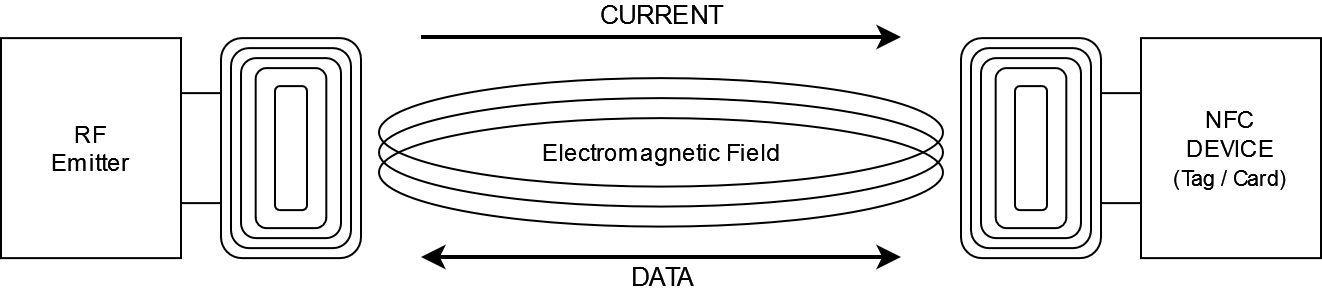
\includegraphics[width=0.9\textwidth]{bignfc}
	\caption{A general view of the NFC connection.}
	\label{fig:nfc_conn}
\end{figure} 

This type of reaction is possible thanks to the inductive coupling mechanism: when two devices are brought close together, the electromagnetic fields generated by their antennas induce in each other a current, which allows a data transfer between the two controllers. For example a common situation would have a card reader (the active device) and a NFC tag (passive device) which holds some data on its memory.\par

It's worth mentioning that the connection formed is weak, and requires the two devices to stay close for the whole operation, which could be considered problematic due to the low transmission speed, averaging under 0.5 Mbit/s. However, in my case but also in general use cases, the weight of data that is being transferred is relatively small, so the close-range connection can be short without causing any kind of loss.\par

I've used different kinds of NFC based devices, which are going to be described in the next sections.\pagebreak

\subsection{MFRC522}

The MFRC522 is an integrated RFID reader/writer module developed by NXP Semiconductors, which is able to interact with RFID cards or NFC compliant devices with a variety of protocols like MIFARE, NTAG or the standard ISO/IEC 14443 Type A. It is widely used in many applications, like identification/access control and data transfer.\par

As mentioned before, it is able to create a wireless connection with NFC tags or cards thanks to the inductive coupling, by taking the active role in the mechanism and inducing a current in the other half of the circuit.\par
\begin{figure}[h]
	\centering
	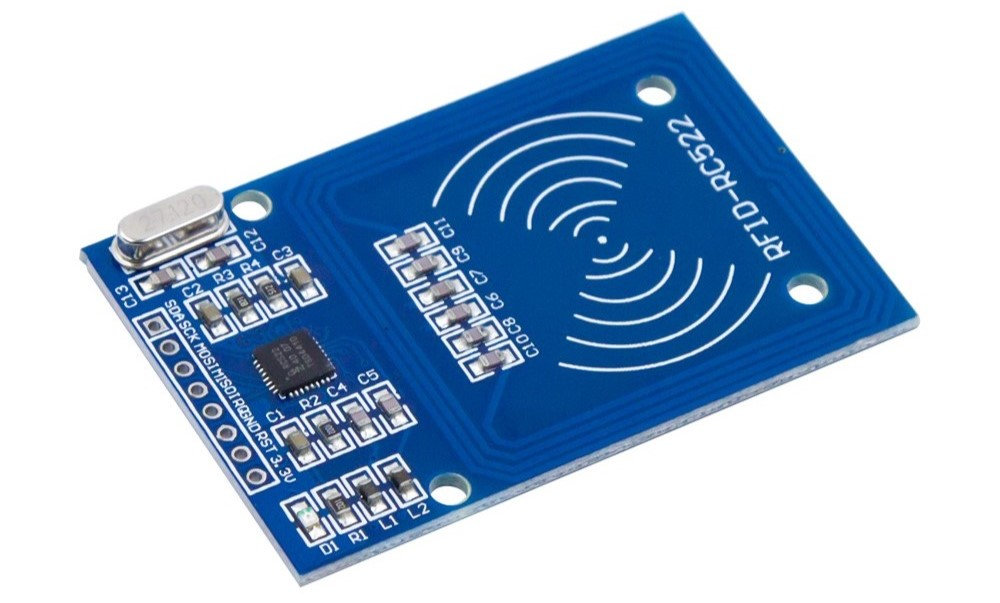
\includegraphics[width=0.4\textwidth]{mfrc522}
	\caption{The MFRC522 module.}
	\label{fig:mfrc522}
\end{figure} 

Using the SPI (Serial Peripheral Interface) Communication Protocol, the RFID module has been paired with different microcontrollers, allowing the system to interface with the NFC tags and cards, in order to read or write data off the EEPROM memory chips.\\
Below, a schematic of the wiring of the ESP boards (ESP32 and ESP8266) I've paired the MFRC522 module with.

\begin{figure}[h]
	\centering
	\begin{minipage}{0.5\textwidth}
		\centering
		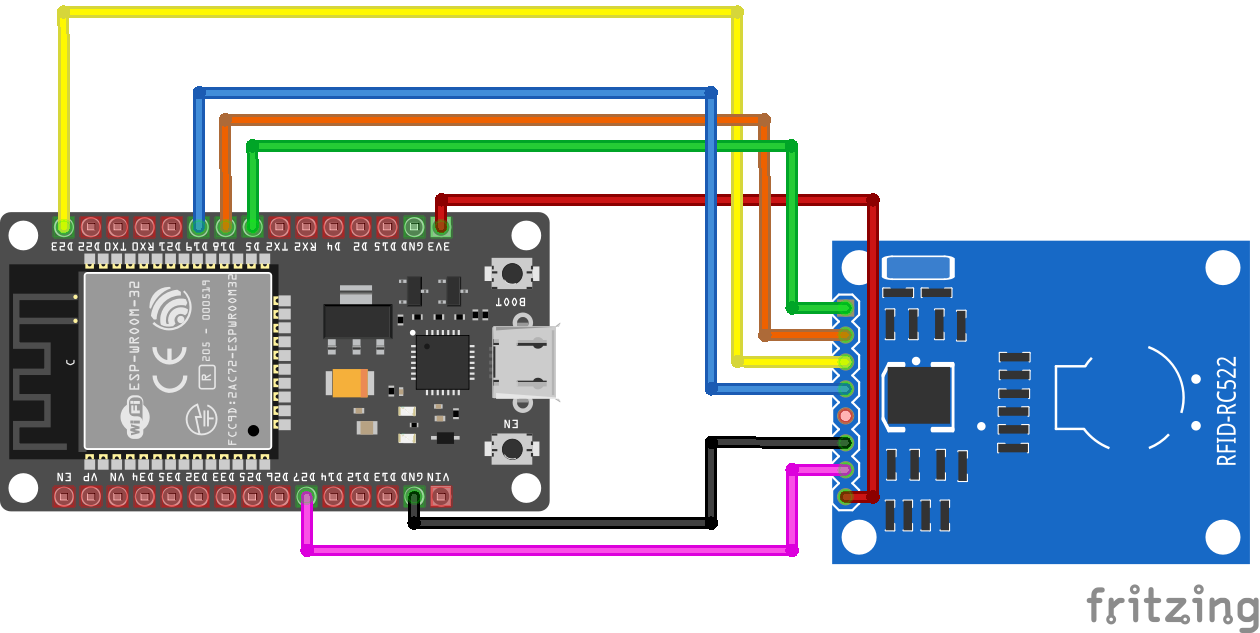
\includegraphics[width=0.9\textwidth]{esp32_mfrc522} % first 
		\label{fig:esp32_mfrc522}
	\end{minipage}\hfill
	\begin{minipage}{0.5\textwidth}
		\centering
		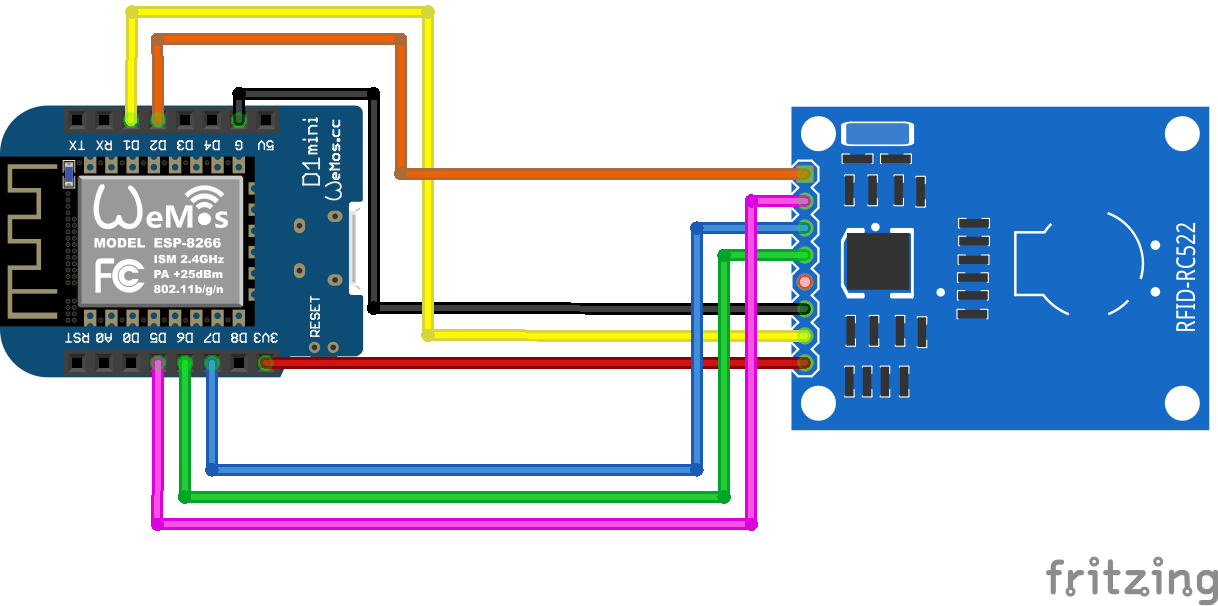
\includegraphics[width=0.9\textwidth]{esp8266_mfrc522} % second 
		\label{fig:esp8266_mfrc522}
	\end{minipage}
	\caption{The wiring diagram of the two boards to the RFID reader, created with Fritzing. ESP32 on the left, ESP8266 on the right.}
\end{figure}

\subsection{NFC Tag - NTAG213}

The NTAG is a type of NFC technology developed by NXP Semiconductors. The same company owns and produces the NTAG series of NFC tags and chips..\\
For this project, the NTAG213 \cite{ntag213} model has been chosen due to their high versatility and their low price, making them perfect for a variety of applications, not to mention their wide availability on online resellers, but the use of another type of tags is not precluded. In fact one model of the same NTAG series, such as NTAG216 would have been a fine replacement. However the former was chosen as it costs less and for this context there was no need for a tag with bigger capacity like the NTAG216 is.

\begin{figure}
	\centering
	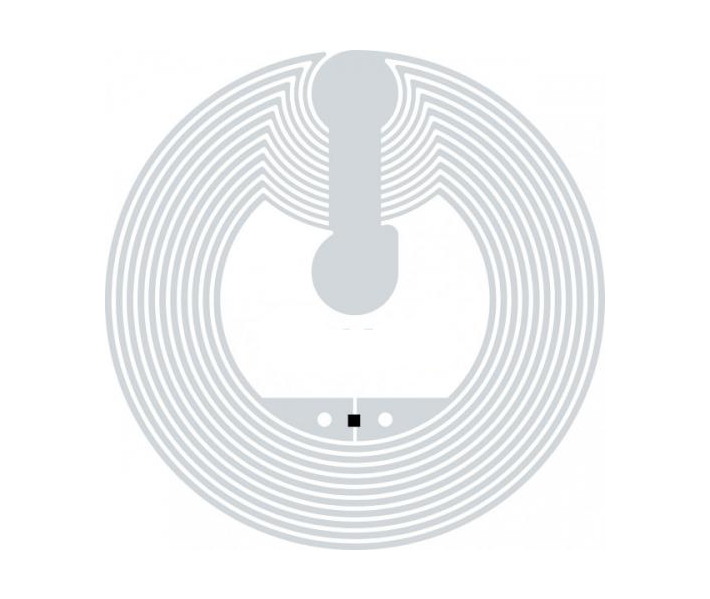
\includegraphics[width=0.2\textwidth]{ntag213}
	\caption{The NFC tag NTAG213.}
	\label{fig:ntag213}
\end{figure} 


The NTAG213 has a memory of 180 bytes, organized in 45 pages with the size of 4 bytes per page. It has a data structure that leaves 36 pages (144 bytes) available for user data, while the other pages are used for metadata, configuration and security.
NTAG213 tags are designed to fully comply to NFC Forum Type 2 Tag (Ref. 2) and
ISO/IEC14443 Type A (Ref. 1) specifications.

\begin{figure}[h!]
	\centering
	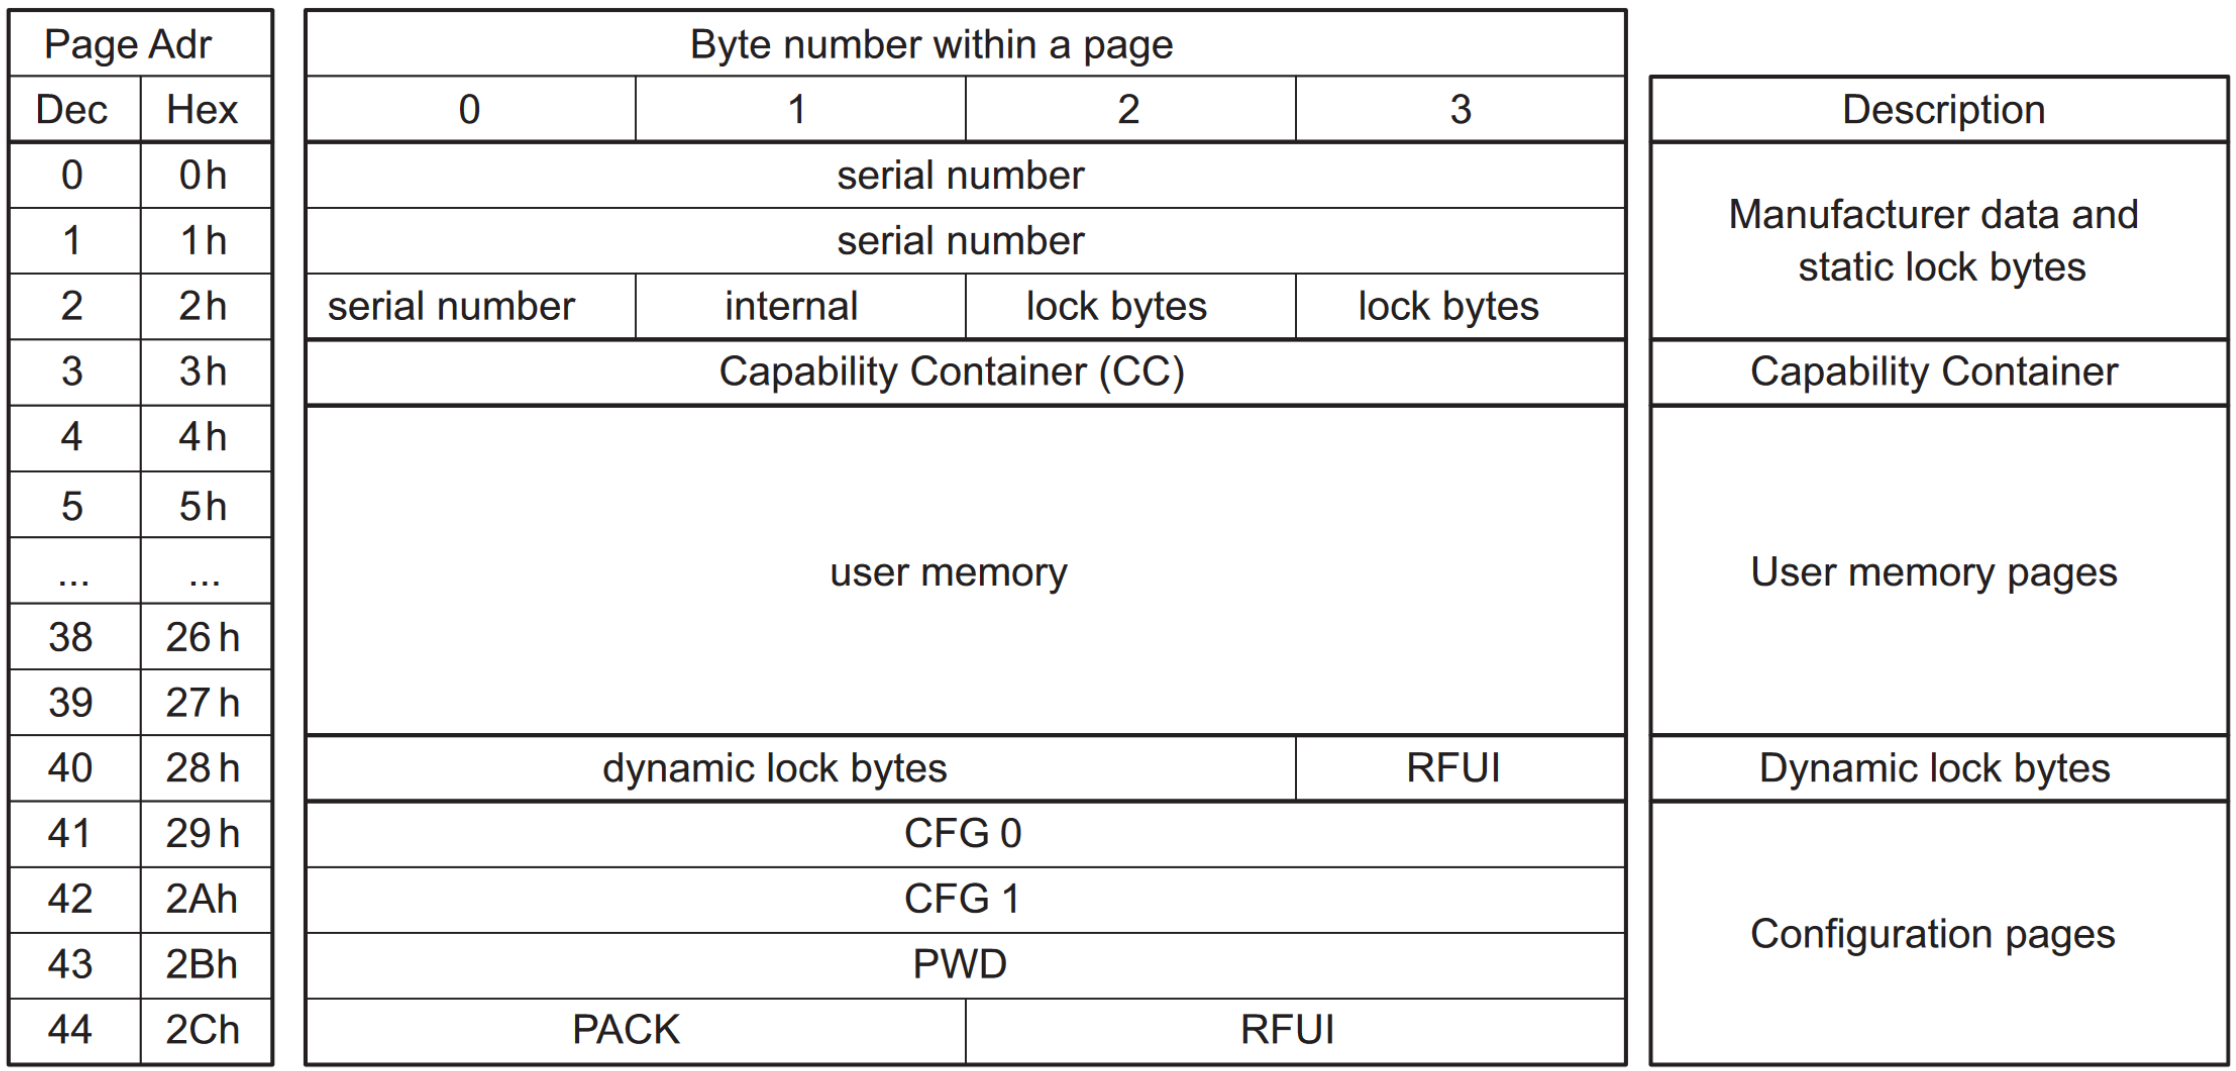
\includegraphics[width=1.05\textwidth]{ntag213memory}
	\caption{The memory organization of NTAG213.}
	\label{fig:ntag213memory}
\end{figure}

As it's possible to see from the table, the first 3 pages (0x00 - 0x02) contain the serial number of the chip and lock bytes, in page 0x04 to 0x27 there is the memory assigned to the user (where the UID of the registered customer is stored) and then the last pages, from 0x28 to 0x2C contain bytes dedicated to the configuration and security. 


\subsection{NFC Card - MIFARE Classic 1K}
MIFARE is the NXP Semiconductors-owned trademark of a series of chips widely used in contactless smart cards. 

The MIFARE Classic 1K \cite{mifare1k} was chosen since, as their counterpart mentioned in the section before, are also pretty cheap and as easy to find on online shops, making them an ideal technology to work with.
\newpage

\begin{figure}
	\centering
	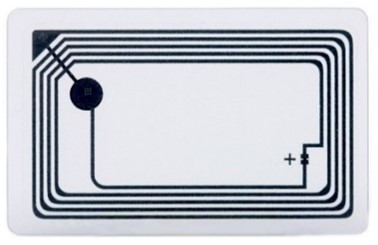
\includegraphics[width=0.3\textwidth]{mifare1k}
	\caption{The NFC card MIFARE 1K}
	\label{fig:mifare1k}
\end{figure} 

This card's 1024 byte memory is organized in 16 sectors of 4 blocks each, and each block has 16 bytes. In each sector, the last block is called Sector Trailer Block, and is reserved for data such as the Secret Keys A and B, and the Access Bits, which represent the access conditions to the sector.

\begin{figure}[h!]
	\centering
	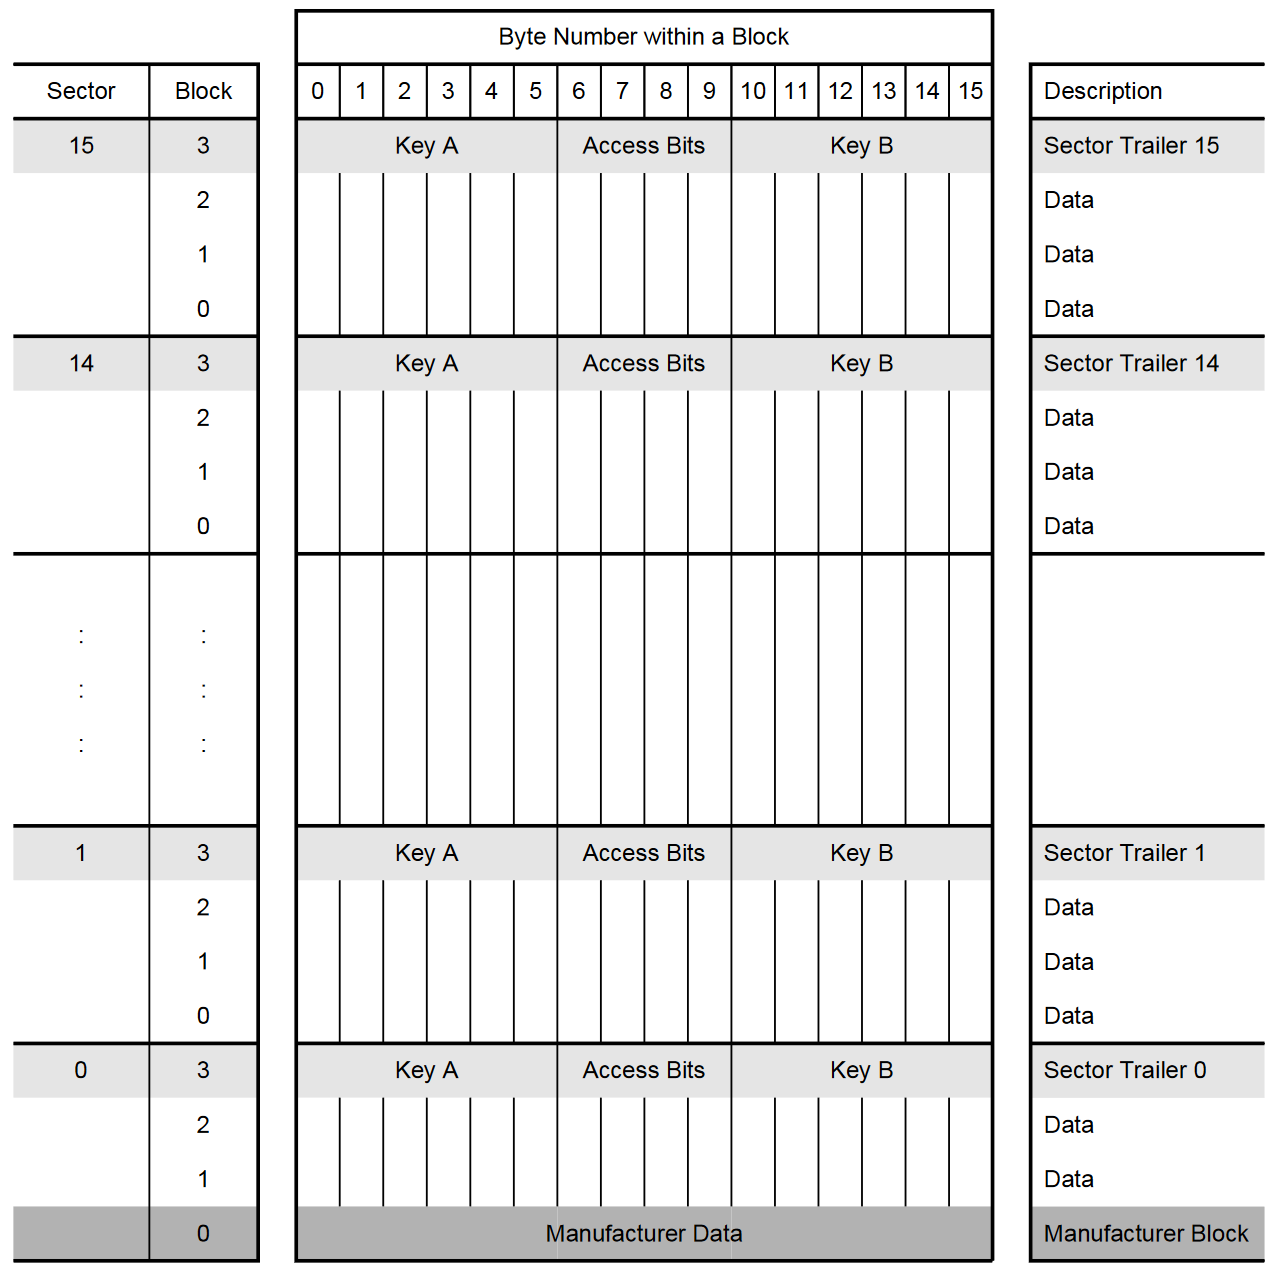
\includegraphics[width=0.8\textwidth]{mifare1kmemory}
	\caption{The memory organization of MIFARE Classic 1K.}
	\label{fig:mifare1kmemory}
\end{figure}

Every sector (00 - 15)  contains a Sector Trailer Block (03), which leaves the first three blocks (00 - 02) to store user data, with an exception for the first sector, which uses also its first clock to store manufacturer data.
Inside the Sector Trailer Block, the Secret Keys A and B take respectively the first and last 6 bytes of the block, while the 4 bytes left are assigned to the Access  Bits.

\subsubsection{Common Uses}
This particular model of NFC card is commonly used for numerous services that require a card; in fact most of the population probably carries one in their wallet.

For instance, many students attending at UniUD joined the CUS (a sport association that offers the students many options to partake in some sportive activities). The card which the students receive, also used to access many structures, is in fact a MIFARE 1K model and in the fifth chapter of this thesis, which discusses the security aspects needed to be implemented, I will try to explain why and how it bears some security flaws.


\subsection{ESP 32}
ESP32 is a product of Espressif Systems, designed for development and simple projects where a power efficient processor is needed, but also a wide compatibility with electronics, thanks to the GPIO pins. The board also integrates 2.4 GHz WiFi and Bluetooth connectivity, which is very useful for IoT uses.
The term ESP32 is often used to refer to the whole development board for simplicity, but it actually is the \textbf{MCU} (\emph{MicroController Unit}) soldered on the board.

This board was used to connect the MFRC522 device (through the SPI interface) in order to read the NFC tags present in the glasses.
Once it detects a NFC tag, after checking for the the user ID, it sends and order to another board to activate the pump and later, to stop it.

Instead of the ESP8266, this board was used, as it typically offers a better performance than its counterpart. As the code constantly checks for new NFC tags and needs to quickly check their memory, a more stable and performant board is more suited for the job.

\begin{figure}[h!]
	\centering
	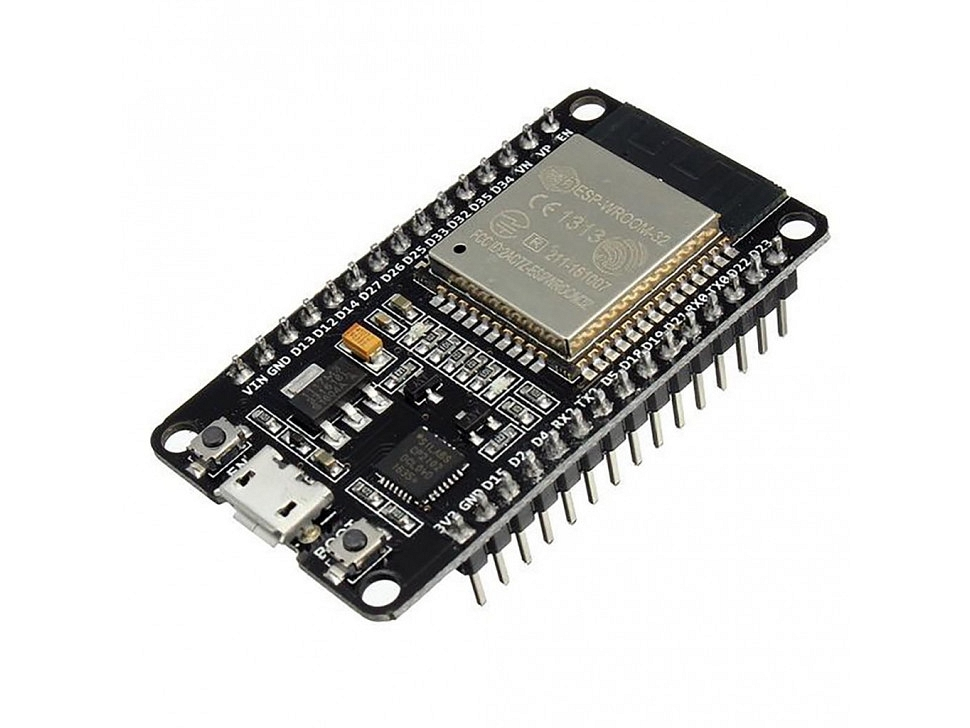
\includegraphics[width=0.3\textwidth]{esp32}
	\caption{The ESP32 board.}
	\label{fig:esp32}
\end{figure} 

\subsection{ESP8266}
ESP8266 is another MCU owned by Espressif Systems, also commonly seen in the development of IoT projects. The  model used, WEMOS D1 mini, offers a smaller board with less GPIOs, but keeps the same specifics and capabilities of the ESP8266 processor. This device was used in two different cases:
\begin{itemize}
	\item For the activation of the pump (formerly, the OLED display), controlled by the ESP32. Since the pump only has 2 connectors for the current and none for any other kind of digital signal, there is a need of an external relay to activate it.
	\item For the transfer of the User ID from the user's personal card to the NFC tag inside the glass.
\end{itemize}

\begin{figure}[h!]
	\centering
	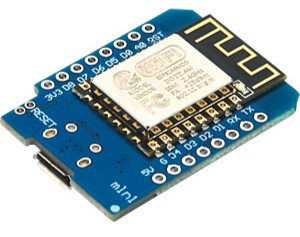
\includegraphics[width=0.3\textwidth]{esp8266}
	\caption{The ESP8266 board.}
	\label{fig:esp8266}
\end{figure} 

\subsection{Peristaltic Pump}
At the beginning of the project, the pump has been replaced by a simple 0.96" OLED screen that can mimic the pump's state (idle/working), and provide other information.

\begin{figure}[h!]
	\centering
	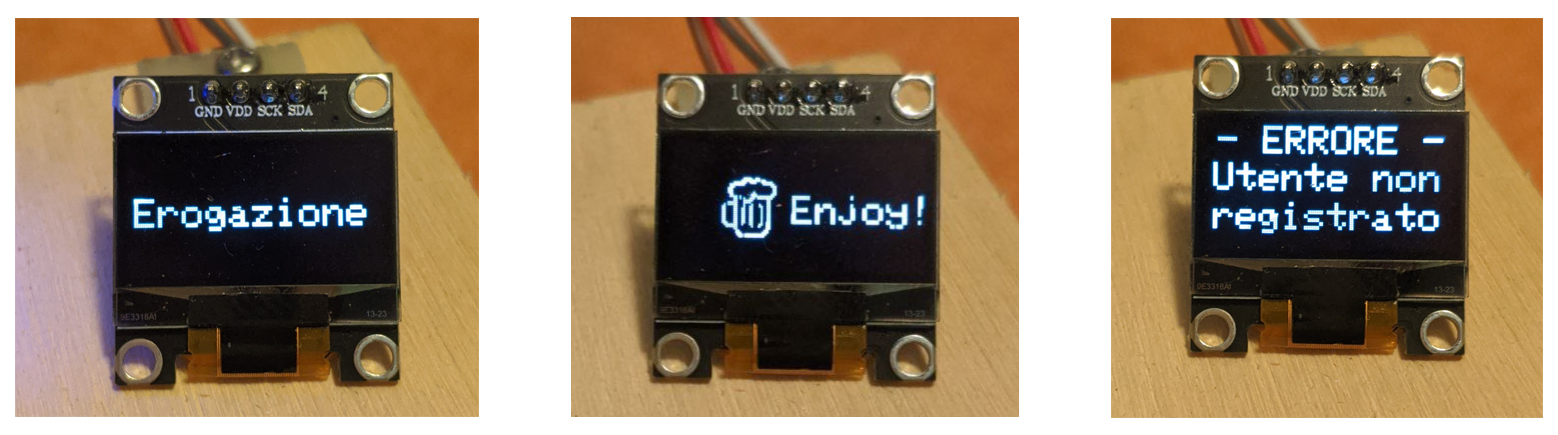
\includegraphics[width=.85\textwidth]{screen_status}
	\caption{The OLED screen in three states: dispensing a drink, showing a successful transaction and showing an error message.}
	\label{fig:enjoy_screen}
\end{figure}

 In the final stages, the pump has been actually implemented alongside the screen. The type used consists in a  peristaltic pump, as it's the best choice to actually build a working prototype/mockup. The pump model works on 12V at 5W, so an external power source and transformer is needed, as nor the development boards (ESP boards), Raspberry Pi, or PC's USB port can supply that kind of current.
 
\begin{figure}[h!]
	\centering
	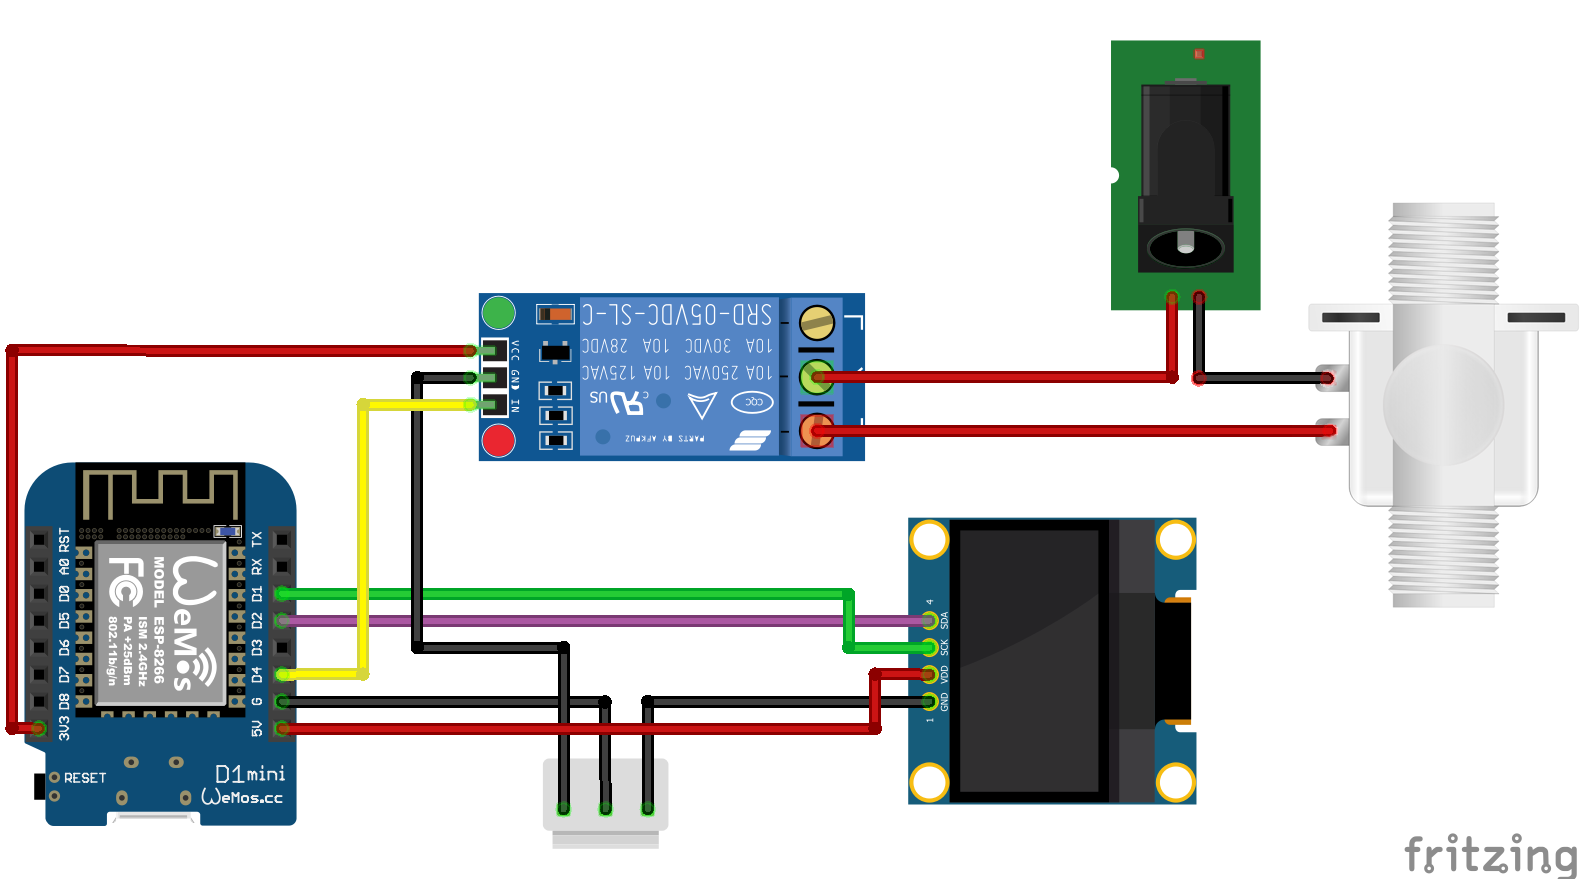
\includegraphics[width=0.7\textwidth]{esp8266_pump_screen}
	\caption{The wiring of the ESP module with the pump and OLED screen.}
	\label{fig:pump}
\end{figure}

\newpage

\subsection{Raspberry Pi}
The Raspberry Pi is a series of small and affordable computers developed by the Raspberry Pi Foundation. It is a fully functioning computer aimed to promote learning, experimentation and development of projects that vary in complexity. It runs on Raspbian OS, a lightweight fork of Linux, and the boards offer a vast array of connectivity thanks to the GPIO pins, USB ports and wireless connection \cite{raspberrypi}.\\ \\
For the project, a Raspberry Pi model 3A+ was used, which I already owned and used for other different experiments.
It serves as the host of the MQTT broker that accepts and forwards messages to the connected clients.
It also hosts the Python program which subscribes to the above mentioned broker in order to receive the requests of the ESP32 boards to activate the pump.

\begin{figure}[h!]
	\centering
	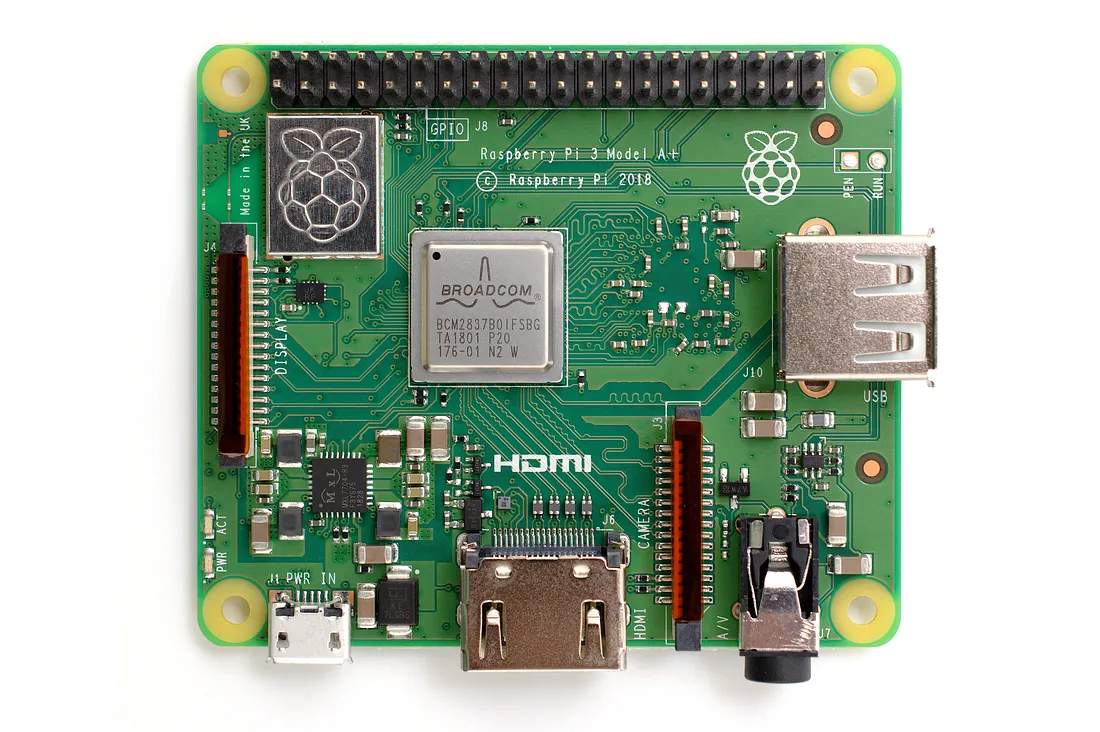
\includegraphics[width=0.4\textwidth]{raspberrypi3a+}
	\caption{The Raspberry Pi model 3A+.}
	\label{fig:raspberrypi}
\end{figure} 

\subsection{Server}

A computer is designated to host the project's database and a PHP API is used to interact with it from the application.
Originally, the Raspberry Pi was used to host all the software components, but even though this particular module is capable of sustaining the workload of all the components, later it has been decided to split the work on two different machines.

If using a single machine would have worked for a simple demonstration in the early development stages, it wouldn't be a proper solution in a more advanced deployment: while the number of stations which dispense drinks is relatively small -probably not over 10-, the number of active users on the application, sending multiple requests to the API is potentially much bigger.

This is why the Raspberry Pi was tasked with the internal job of managing the requests from the stations, while giving the job of responding to the users requests to another scalable system (in this case, a PC acting as a server).
\newpage

\section{Software}

In this section all the software components and technologies used to accomplish the realization of this project are going to be showcased and it will be explained how they connect to each other.

\subsection{MQTT}
MQTT (Message Queuing Telemetry Transport) \cite{mqtt}, is a lightweight messaging protocol often used in environment with low bandwidth and where the payload is relatively small, which is why it's commonly used in the Internet of Things field, where efficient and real-time communication is often required but also the network often present connection problems, thus needing the clients to reconnect seamlessly.

The protocol, built on the \emph{Publish and Subscribe} model, involves the use of a central device called \textbf{Broker}. The clients connect to this device and can publish data (Publisher) on a certain topic or subscribe to it to receive (Subscriber) relevant data. In this paradigm, both Publishers and Subscribers are considered clients that interact with the Broker, which will act as intermediary between them.

One of MQTT's key aspects revolves around the ability of multiple clients to publish/subscribe to the same topic (which acts as a categorized channel), this way multiple clients can subscribe to the same topic and consume the received data without worrying about concurrency; instead of an 1:1, it's possible to establish a N:N communication.

Another important aspect of the protocol is the support for different levels of \emph{Quality of Service} to ensure the messages reliability. Depending on the application context, a message can be published without needing any kind of feedback from the broker on whether it has been received or not (\emph{fire-and-forget}), or depending on the QoS level, the broker stores the message to ensure its delivery at least/exactly once.

Lastly, as it will be explained in the late chapters, MQTT supports an authentication mechanism and can be secured through SSL/TLS.

\subsection{Arduino IDE}

In order to program the microcontrollers of the ESP boards, an application like Arduino IDE was used to write and load the programs files on their memory.\\

Arduino IDE is an open source software for the developing, compiling and uploading of code to compatible microcontrollers and development boards.
Arduino allows to write code for these boards (sketches) in a simplified version of C/C++, using case-specific libraries to help the board interact with modules or execute specific instructions. 

Arduino IDE allows to use third-party platform packages, making a variety of different boards compatible: this applies to the project's scenario, where in order to utilize the ESP32 and ESP8266 boards multiple libraries and files were installed in the environment \cite{esp_install_arduino}.

Among the more common libraries used with kind of boards, like Wifi.h, SPI.h, etc., one in particular is required to interface the microcontrollers with the MFRC522 RFID module. After searching different repositories, I've found one on GitHub that provided a few functions and data structures to interact with the NFC devices: MFRC522.h \cite{mfr522library}.\\
Unfortunately this library doesn't seem to be maintained so often anymore, but it has provided adequate support for the growth of the project. During the development it caused little trouble using it, with minor inconveniences that have been easily overcome. For example, 
in multiple instances a function tailored for the model MIFARE Ultralight C, was used to communicate with the NTAG213. This is possible because the two chips have a very similar structure, allowing sometimes to use the same functions for both.

It allows the RFID module to interact with most of the cards according to the ISO/IEC 14443 standard, but in order to better understand how this library works, a visual aid is first needed to illustrate the aforementioned ISO standard.

\subsubsection{ISO/EIC 14443}


The ISO/IEC 14443 standard \cite{wiki:iso14443} is a four-part international standard for contact-less smart cards operating at 13.56 MHz in close proximity ($\sim$ 10 cm) with a PCD (Proximity Coupling Device, aka a Contactless Reader), and was developed jointly by the International Organization for Standardization (ISO) and the International Electrotechnical Commission (IEC).\cite{iso14443}\\ This standard describes the modulation and transmission protocols between card and reader to create interoperability for contact-less smart card products. There are two main communication protocols supported by the ISO/IEC 14443 standard, they are addressed as Type A and Type B. \cite{nfc-tools}\par

The parts of the standard can be summed up as it follows \cite{an10833}:

\begin{itemize}
	
	\item ISO/IEC 14443-1 : Defines the physical size of compliant PICC and antennas.
	\item ISO/IEC 14443-2 : Defines the frequency, the modulation and coding.
	\item ISO/IEC 14443-3 : Defines the start of the communication and how to select the PICC (initialization and anti-collision sequence).
	\item ISO/IEC 14443-4 : Defines the protocol for data exchange between PCD and PICC.
\end{itemize}
The parts 2 and 3 are split in Type A and B, creating two variants of the standard, ISO/IEC 14443 Type A and ISO/IEC 14443 Type B.\\The MIFARE Classic 1K and NTAG213 are both compliant to the variant Type A.\\
Before exchanging data, it is necessary to establish a connection and determine compatibility between PCD (i.e. MFRC522) and a chip's PICC. \\The part 3 and 4 of the standard describe this process, and can be summed up as this set of procedures:
\begin{enumerate}
	\item The PCD polls for PICCs in the field, by sending a broadcast of command REQA (REQuest command, Type A). \\The initial state of a PICC is \textbf{IDLE}, meaning that is not ready yet to communicate.
	\item When a PICC is within the operating range of the PCD and receives the REQA, any compatible PICC responds and returns the ATQA (Answer To reQuest, Type A). The ATQA buffer contains information about the chip, for example the UID size.\newline This changes the chip's \textbf{IDLE} state to:
	\begin{itemize}
		\item \textbf{READY 1} if the chip is a NTAG213.
		\item \textbf{READY} if the chip is a MIFARE Classic 1K.
	\end{itemize}
	
	\item The following phase of communication, known as \emph{cascade level 1} involves the PCD sending a "SELECT CL1" command to the PICC, which will resolve the first part of his UID. \\This changes the chip's \textbf{READY 1} state to \textbf{READY 2}.
	\item In this state, the PICC supports the NFC reader in resolving the second part of its UID with the \emph{cascade level 2} "ANTICOLLISION" command.\\
	Once again, the PICC issues another command, this time being "SELECT CL2" and the state is changed from \textbf{READY 2} (or \textbf{READY} for the MIFARE Classic 1K) to \textbf{ACTIVE}.
		
\end{enumerate}

\begin{figure}[h]
	\centering
	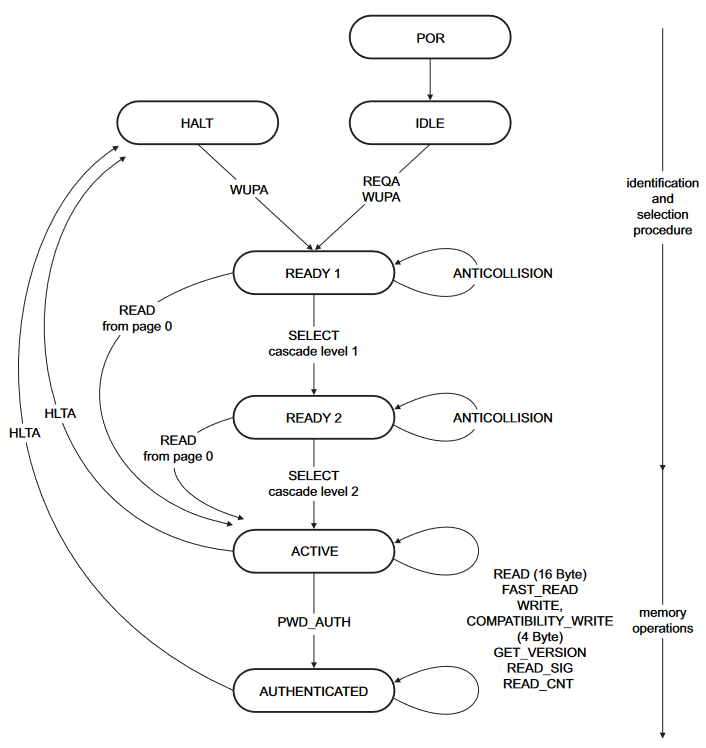
\includegraphics[width=0.80\textwidth]{nfcsequence}
	\caption{A graph of the sequence.}
	\label{fig:nfcsequence}
\end{figure} 
There has been a distinction between the two types of NFC supports since NTAG213, among other necessities, needs to cycle through the same operations twice to resolve his UID. The maximum chunk length which is exchanged after a SELECT command, is 4 bytes. The NTAG213's UID is 7 bytes longs, needing a first transfer of 3 bytes followed by the second one containing the last 4 bytes.\\ \\
Now the NFC devices are ready to communicate and use memory operations such as READ and  WRITE.

The MFRC522.h library provides these instructions through two functions calls, PICC$\_$IsNewCardPresent() and PICC$\_$ReadCardSerial().

\subsubsection{PICC$\_$ IsNewCardPresent()}

\begin{lstlisting}[language=C++,style=cpp,caption={PICC$\_$ IsNewCardPresent().}]
bool MFRC522::PICC_IsNewCardPresent() {
	 byte bufferATQA[2];
	 byte bufferSize= sizeof(bufferATQA);
	
	 // Reset baud rates
	 PCD_WriteRegister(TxModeReg, 0x00);
	 PCD_WriteRegister(RxModeReg, 0x00);
 	
 	 // Reset ModWidthReg
	 PCD_WriteRegister(ModWidthReg, 0x26);
	
	 MFRC522::StatusCode result= PICC_RequestA(bufferATQA, &bufferSize);
	 return (result == STATUS_OK || result == STATUS_COLLISION);
} 
\end{lstlisting}
This function creates a byte array bufferATQA used to store the PICC's reply to a REQA command issued by the PICC$\_$RequestA function.\\
At the end of this function, if the REQA command has success, the PICC state will become \textbf{READY} and a \emph{STATUS$\_$OK} value will be returned, otherwise it will return \emph{STATUS$\_$COLLISION}.

\subsubsection{PICC$\_$ ReadCardSerial()}

\begin{lstlisting}[language=c++,style=cpp,caption={PICC$\_$ReadCardSerial().}]
bool MFRC522::PICC_ReadCardSerial() {
	MFRC522::StatusCode result = PICC_Select(&uid);
	return (result == STATUS_OK);
} 
\end{lstlisting}
This function is a wrapper for the PICC$\_$Select() function, which brings the PICC state from \textbf{READY} to \textbf{ACTIVE}, and stores the the size and value of the chosen PICC in the \emph{uid} struct.
It returns true if an uid could be read.


\newpage
\subsection{Database}

In order to store new orders, update the users information, retrieve data about the available beers, and other important actions, the system needs to implement an efficient storage which keeps track of the relation among the various entries and acts accordingly. For the project, a relational database for storage is the most adequate solution as the relations between the entities can be proven quite useful. Due to the familiarity with this product and its fairly efficient and simple structure to work with, MySQL has been chosen as the Relational Database Management System.
\\
The database is structured of 4 tables: \emph{Utente} (with email, password and id among their attributes), \emph{Consumazione} (representing and distinguishing each time a user actually used the refilling station, indicating the date, cost, ... ), \emph{Birra} (the beers stored in the database, complete of  name, price per milliliter, type, ... ) and \emph{Pompa} (which links each pump to a specific type of beer).

\begin{figure}[h!]
	\centering
	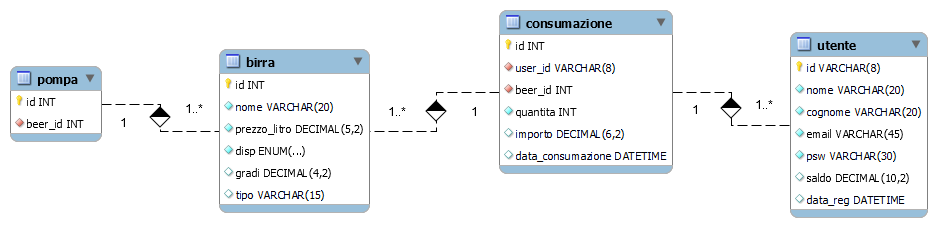
\includegraphics[width=0.95\textwidth]{ER}
	\caption{An ER diagram, showing the tables of the database.}
	\label{fig:dbtables}
\end{figure} 

Upon the execution of certain queries on the database a number of triggers activates and assists the insertion of new information:
\begin{itemize}
	\item \emph{ifDateNull}: If upon registration of a new user, the date field is empty, the DBMS will use the NOW() SQL function to give the entry an appropriate value.
	\item \emph{UpdateImporto}: When a new entry for the table \emph{Consumazione} is added, the system takes its cost and adds it to the user total amount due.
	\item \emph{utenteBeforeInsert}: Upon registration, if the id field has been left empty, the system creates a new randomly picked available id and attributes it to the entry.
\end{itemize}


\subsection{Python Server}
At the core of this project, there is a Python script which is responsible for the interaction between the ESP boards that read the NFC tags, activate the pump and all the queries to the database server, like storing a consumption, checking if the user exists and more.

Its routine is to connect to the MySQL database server, connect to the MQTT broker and stand by, waiting for a new message forwarded by the broker. On receiving a message, it triggers the execution of the callback function onmessage(), which is defined by the MQTT library methods. \newpage
The function, upon the MQTT client receiving a new message, checks its payload's encoding, and acts differently based on the topic the message was retrieved from.

If the topic is "\emph{beer/requests}", then the message comes from a refilling station, and is sending a request to either:
\begin{itemize}
	\item Check if the user is allowed to get the drink, and consequently to activate the pump.
	\item Stop the pump.
\end{itemize} 
The Python script extracts the payload fields \emph{id, idPompa, cmd}, which represent respectively the user's id, the station id that sent the message, and the command it wants to send; then it executes a query on the DB for the user id.
If there's a match, it will send the correct command to the pump through another message published the topic "\emph{beer/pump}", otherwise it will return an error message displayed on the pump's screen (which is also sent using MQTT using the same topic as the successful match).\\

The MQTT client is also subscribed to another topic, "\emph{beer/duration}". This topic is used exclusively by the ESP32 board when the user removes the glass from the NFC reader. The message carries all the information needed to charge the user account for the drink that just got poured: a variable \emph{duration} is used to estimate the volume of the drink. After fetching the corresponding beer id, it inserts the values to the database, which computes the cost of the transaction and stores the entry in the table.




\chapter{Workflow and Use Cases}
In this chapter, the workflow of the main scenarios of a user interacting with the system will be explained in detail, ranging from what happens in each component to the data transmission between them. However, the uses of mobile application, how it's structured and how it interacts with the system will be elucidated in the following chapter.\\

\begin{figure}[h!]
	\centering
	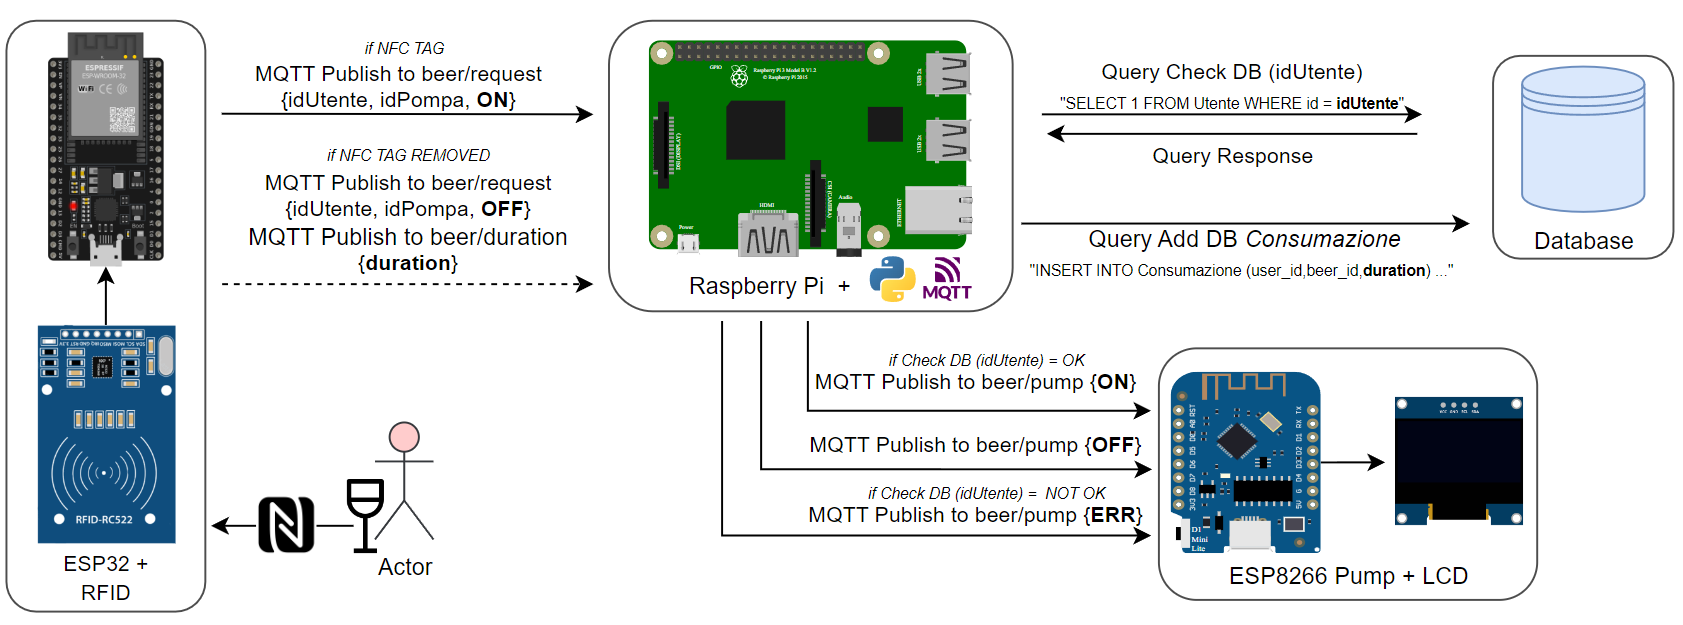
\includegraphics[width=1.05\textwidth]{flow}
	\caption{A general view of the components interactions.}
	\label{fig:flow}
\end{figure} 
This chapter is divided in two parts, respectively regarding the general use case scenario and the detailed explanation of the ESP boards workflow.
\newpage

\section{Overview}
The main use case consists in an already registered user wanting to obtain the beverage: this can be achieved by following two steps: retrieving the NFC enabled glass, and interact with the refill station.


\begin{figure}[h!]
	\centering
	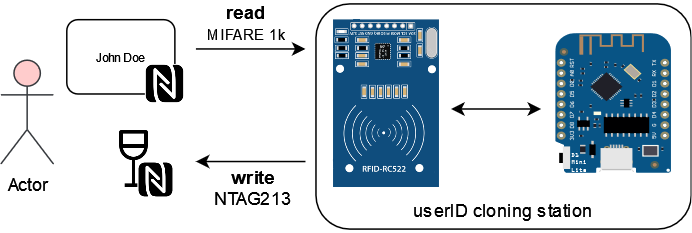
\includegraphics[width=.70\textwidth]{clone}
	\caption{A diagram showing the workflow of the first step.}
	\label{fig:clone}
\end{figure} 
The user needs first to present their personal card, which holds information about their account in the system - their ID number - to a secondary NFC reader. The reader doesn't need to be positioned in any particular position inside the ideal location where the beverage distribution system is located, but it needs to be easily accessed by the users, so a potential candidate spot could be near the dispenser of glasses (of course, not carrying a user ID yet).\\

After the user positions the card on the reader, it will return a visible feedback, whether it holds the user ID, or if there was an error (such as read failure, invalid data structure, memory corruption and, as it will be explained in the following chapters, potentially an invalid authentication password used to read the card). The user then after taking a glass, puts it near the NFC reader which recognizes the device and writes the user ID on its memory: this concludes the first step.\\

Having a glass, the user now can interact with the refill station: putting the glass on the highlighted area under the tap, activates the reader, which reads the ID previously written, and if it meets the conditions, a message to the pump to activate will be sent.

When the user is satisfied with the amount of liquid poured in the glass, by simply lifting it from the surface will prompt the station to send another message to the pump, halting the liquid flow.

With the last action, the system recognizes and charges the user for the amount of liquid poured.
\newpage
\begin{figure}[h]
	\centering
	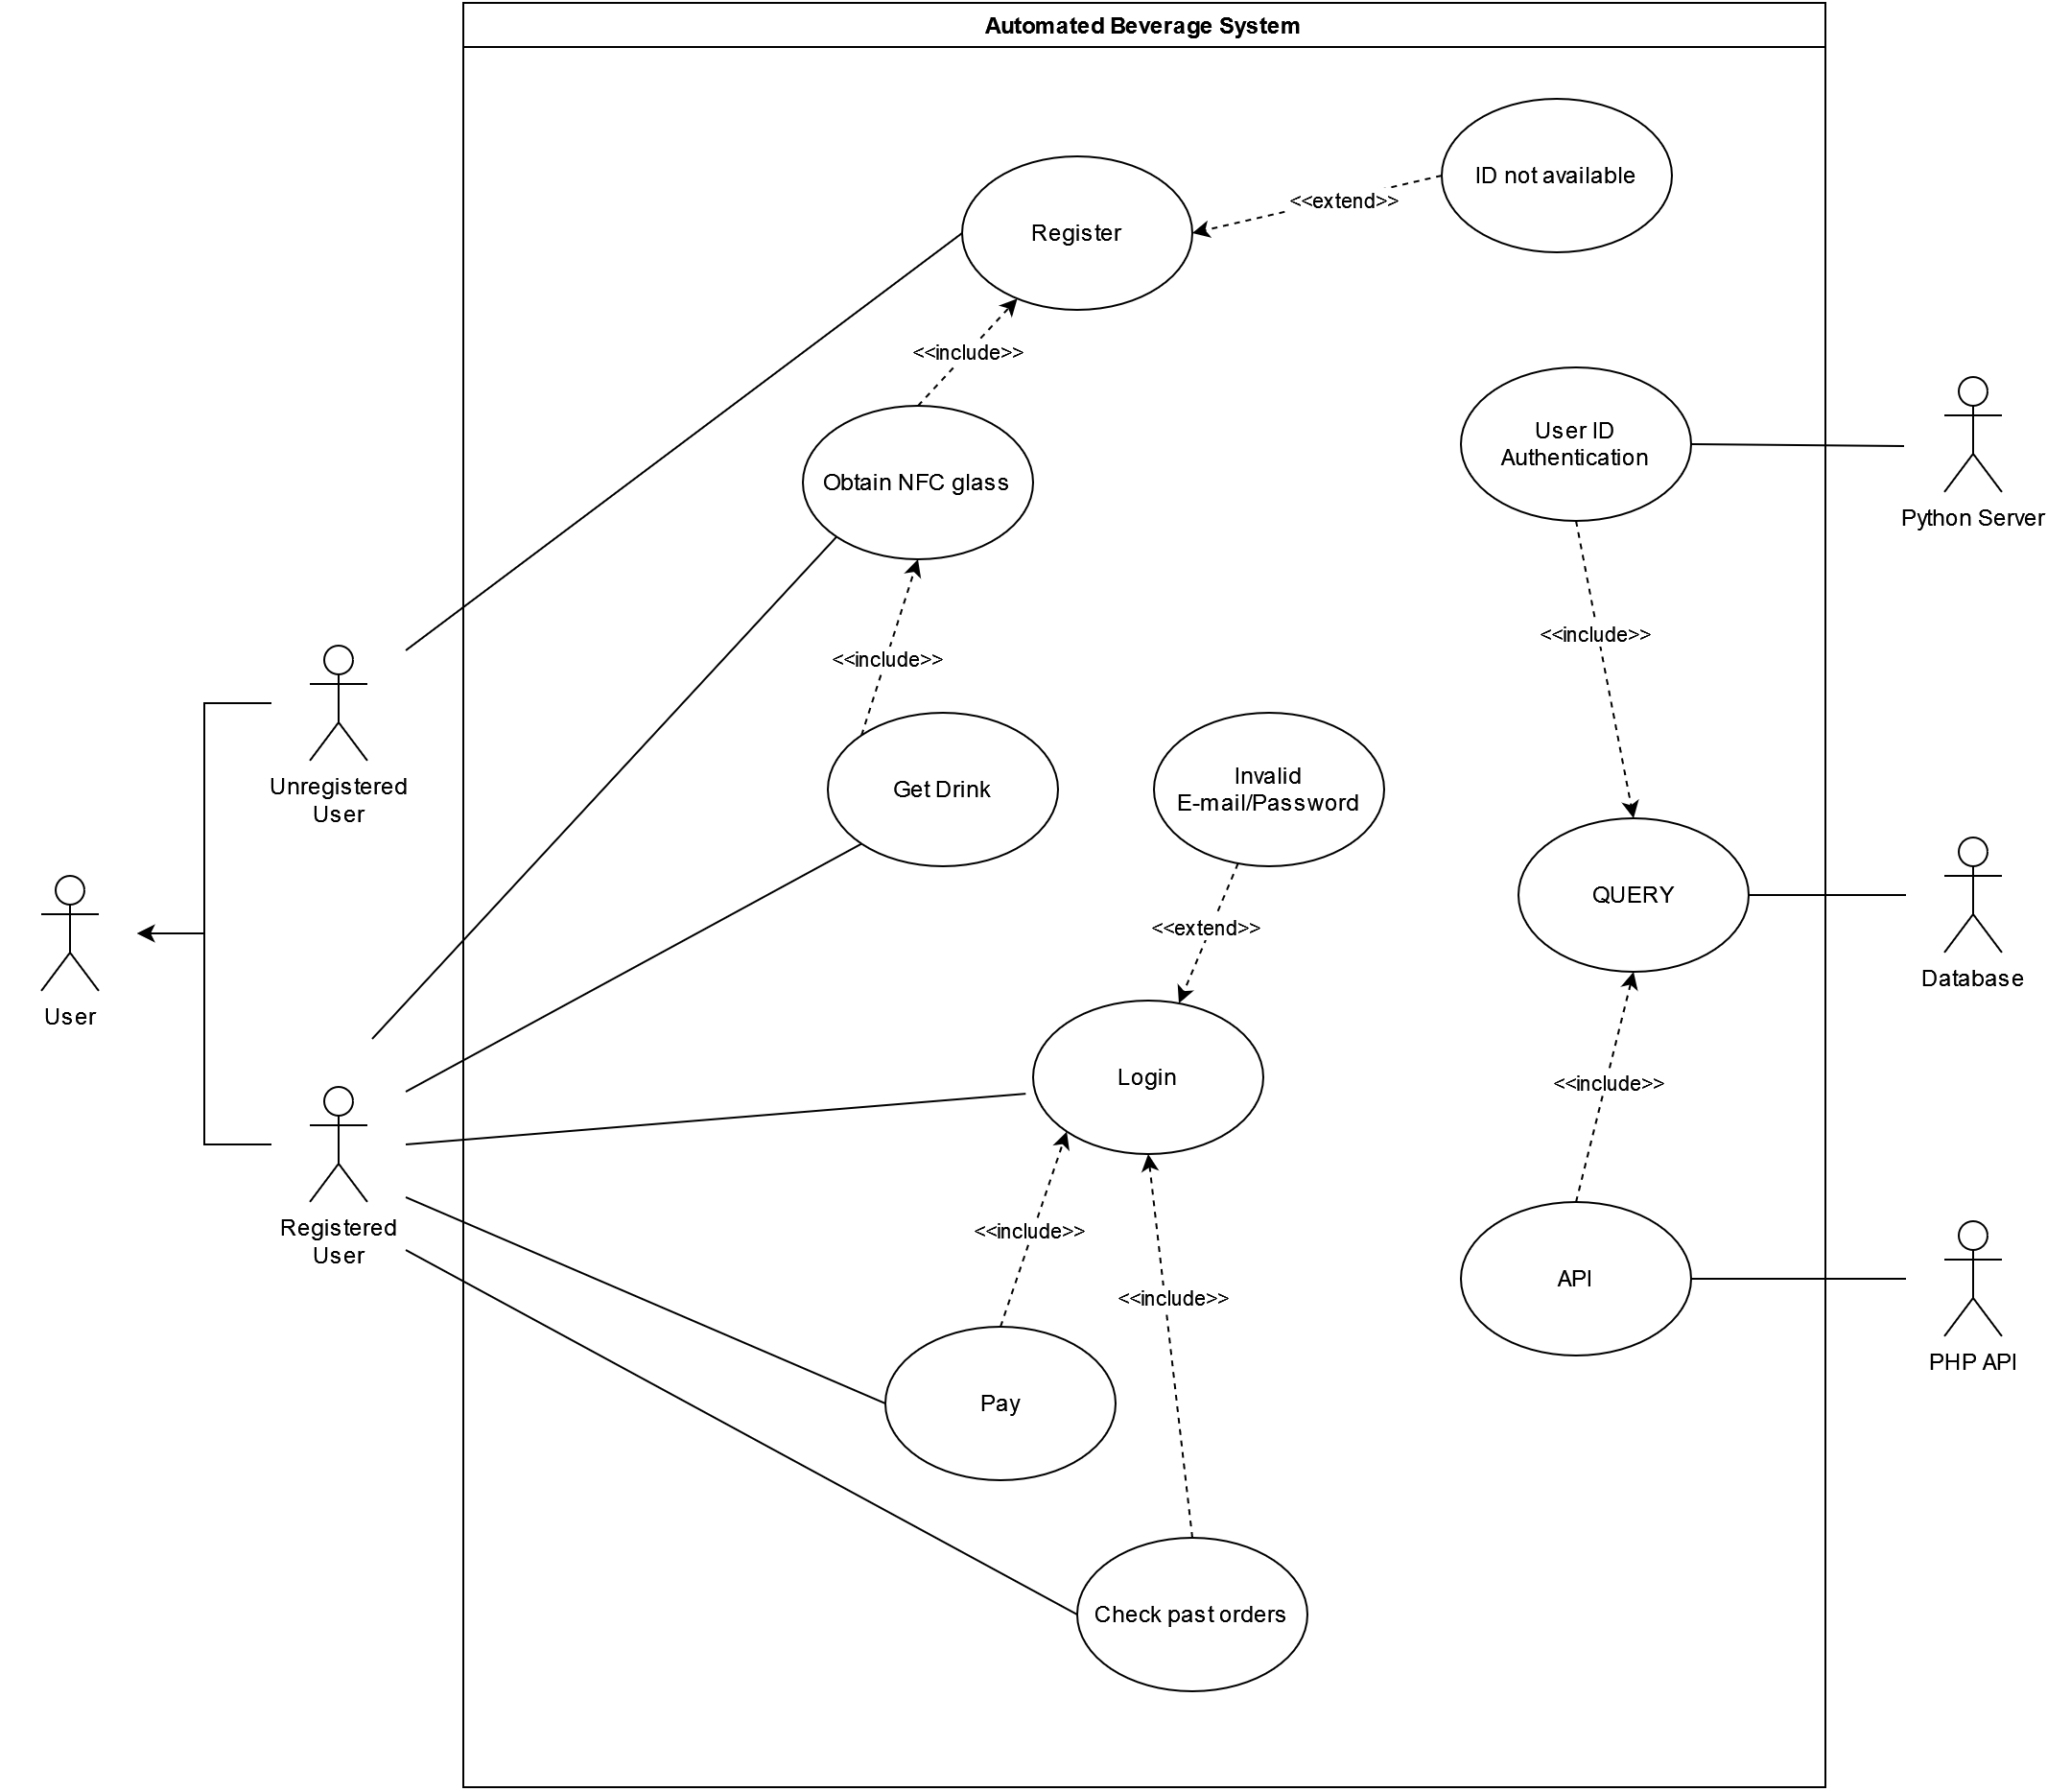
\includegraphics[width=1\textwidth]{usecasediagram}
	\caption{Use Case diagram.}
	\label{fig:usecasediagram}
\end{figure} 

\section{ESP sketches}

The ESP modules used have loaded different sketches, each for a different job with different components to work with. Thanks to their compatibility with a large pool of components, these boards are widely used for many types of application.

There are three programs loaded on the boards: the board that reads a user card and copies their ID on a glass, the one which receives the pump commands, and the one which is responsible of reading the user ID off a glass and publishes the data to a MQTT topic.
\newpage
\subsubsection{Card Reader}

The program is structured so that at the beginning of every loop cycle, it checks for the presence of a new NFC device, using the \emph{isNewCardPresent()} and \emph{ReadCardSerial()} functions, provided by the MFRC522 library. Once a device is placed on the NFC reader, it will read the memory address where the user ID is stored, only if said device is recognized as the correct type of tag.
Then it checks for the value of the \emph{!tagPresent} statement: this variable essentially indicates if the glass is on the reader, if it just got lifted, or if there is no glass.

If the variable is \textbf{false}, it means that it is the first loop iteration where the glass is recognized, thus meaning that it has just been placed, so the program publishes the request to activate the pump (MQTT message to "\emph{beer/requests}") which the Python Server will grant if the user ID in the request is valid. It also sets the value of \emph{tagPresent} to \textbf{true}, and will instantiate a \emph{timeStart} variable with the current time in milliseconds.

The other possible scenario, where a tag is recognized, but the \emph{tagPresent} value is \textbf{true}, implies that the glass has been placed previously, and the user is waiting for the desired amount of liquid before removing it, so the program waits.

If instead, there is no glass placed on the reader, and the first condition equals to \textbf{false}, the program checks for the \emph{tagPresent} value: if it's \textbf{false}, then there is no effectively no glass placed on the reader, but on the other hand, if it is \textbf{true}, then it means that it is the first loop iteration after the glass has been removed. The program calculates the effective duration of the pouring, stops the pump by sending another MQTT message to the same topic, and then sends another one to "\emph{beer/duration}", containing the user ID and the duration, which the Python Server uses to charge the user.

In this particular code, the function PICC$\_$WakeupA() gets executed multiple times, as this brings the PICC to the READY state, since the operations of read/write cause the PICC to exit that state, in order to avoid multiple reads/writes (but in this case it's exactly what it is needed).


\begin{figure}[h!]
	\centering
	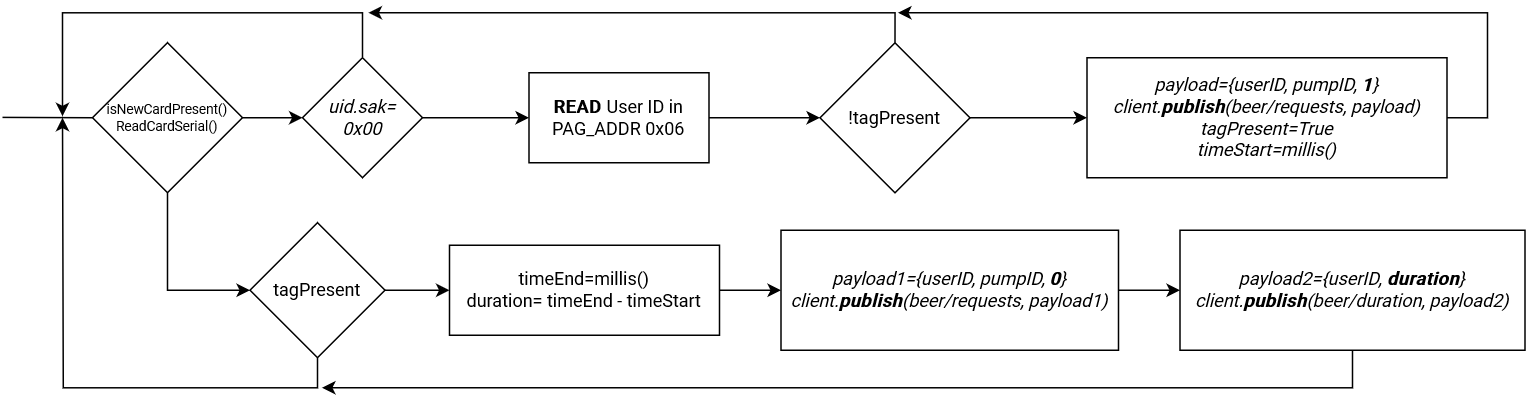
\includegraphics[width=1.0\textwidth]{reader_flow}
	\caption{The flow diagram of the ESP32 board recognizing the NFC enabled glasses.}
	\label{fig:reader_flow}
\end{figure} 
\newpage
\subsubsection{Pump}
The program calls the MQTT client's method \emph{client.loop()} to constantly check for a new message on the subscribed topic, "\emph{beer/requests}". 
Once it receives one, it checks for the command parameter, which represents which command to send to the pump and the correct message to display on the screen. If the other components involved encounter some sort of problem, an error message is displayed on the screen for a couple of seconds.

\begin{figure}[h!]
	\centering
	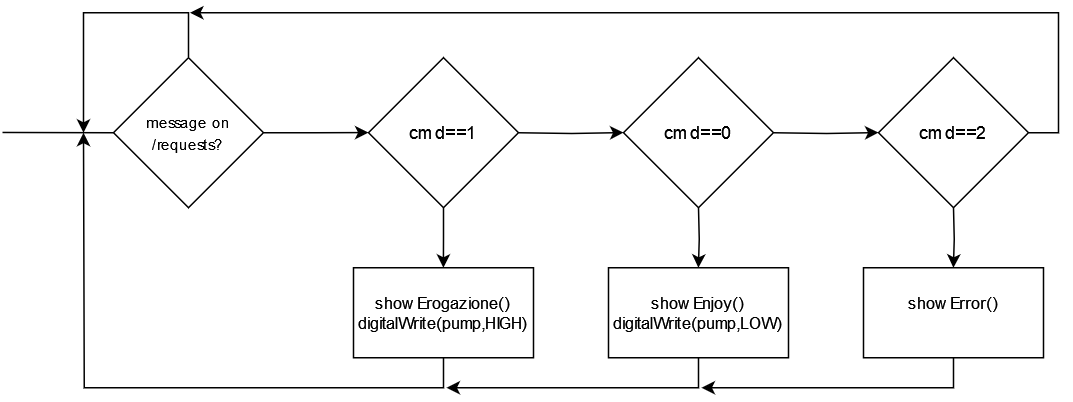
\includegraphics[width=.8\textwidth]{pump_flow}
	\caption{The flow diagram for the ESP8622 board which operates the pump.}
	\label{fig:pump_flow}
\end{figure} 

\subsubsection{User ID cloning}
Again, this program works by constantly checking for the presence of a NFC device: if the presented device is an NFC card, it means the user wants to transfer his ID onto a glass, so it accesses the card's memory and copies the ID value on a specified memory address. If there is instead a NFC tag, after checking that there is an already stored user ID in memory, it writes that value on the tag.

\begin{figure}[h!]
	\centering
	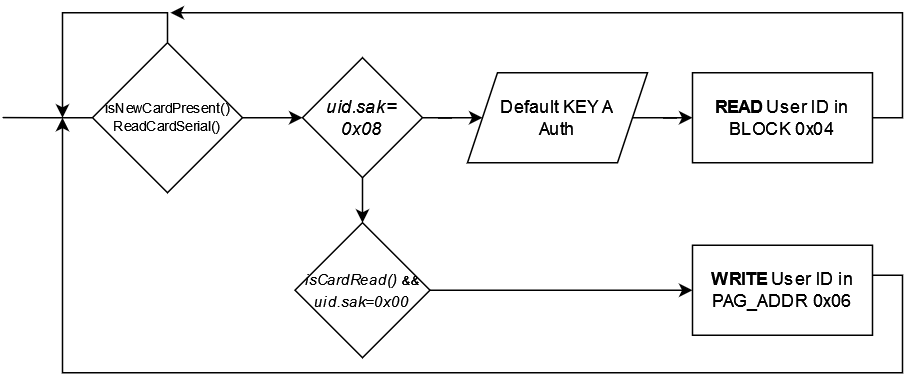
\includegraphics[width=.8\textwidth]{clone_flow}
	\caption{The flow diagram of the ESP8266 board responsible of copying the user ID from the card to the tag.}
	\label{fig:clone_flow}
\end{figure} 




\chapter{Android Application}
To help the interaction between a user and the system, a mobile application has been developed which provides useful information and an authentication mechanism.
The app supports a registration process that allows the user to create an account that will allow the system to track their purchases and after this the user can login using their credentials.
Once logged in, the user is welcomed by a simple homepage screen that redirects to the history of their orders or to the payment page.

\section{Flutter}
Flutter \cite{flutter} is an open-source UI framework developed by Google that allows developers to build multi-platform applications from a single code source. Its core components are the Flutter Framework, providing a set of pre-designed widgets, styles and components for building user interfaces, and Dart, the programming language at the base of the framework. 
The general idea is to create different widgets stacked on top of each other, that behave in different ways under certain circumstances or events, and display them like pages.\\

The mobile app used by the users to check their recent orders, the total due and retrieve other information about their experience with the system, was written using Flutter.
Even though I never had the chance to create a mobile application, its features like hot-reload and a general user friendly approach were a great help to build this application. 

\section{Application and Screens}


On startup, the application presents the option to login or register: either way, the software takes the data entered in the forms, and performs an HTTP request to an API written in PHP to execute a query to the server, checking if either the user already exists and their credentials matches the ones on the server, or in the case of the user trying to register, if the credentials are already taken, prompting then to try with different ones in such occurrence.\\
If the user is trying to login with non matching credentials, or if they are trying to register with non-available ones, a message pop up will appear, reporting the issue.
\newpage

\begin{figure}[h!]
	
	\centering
	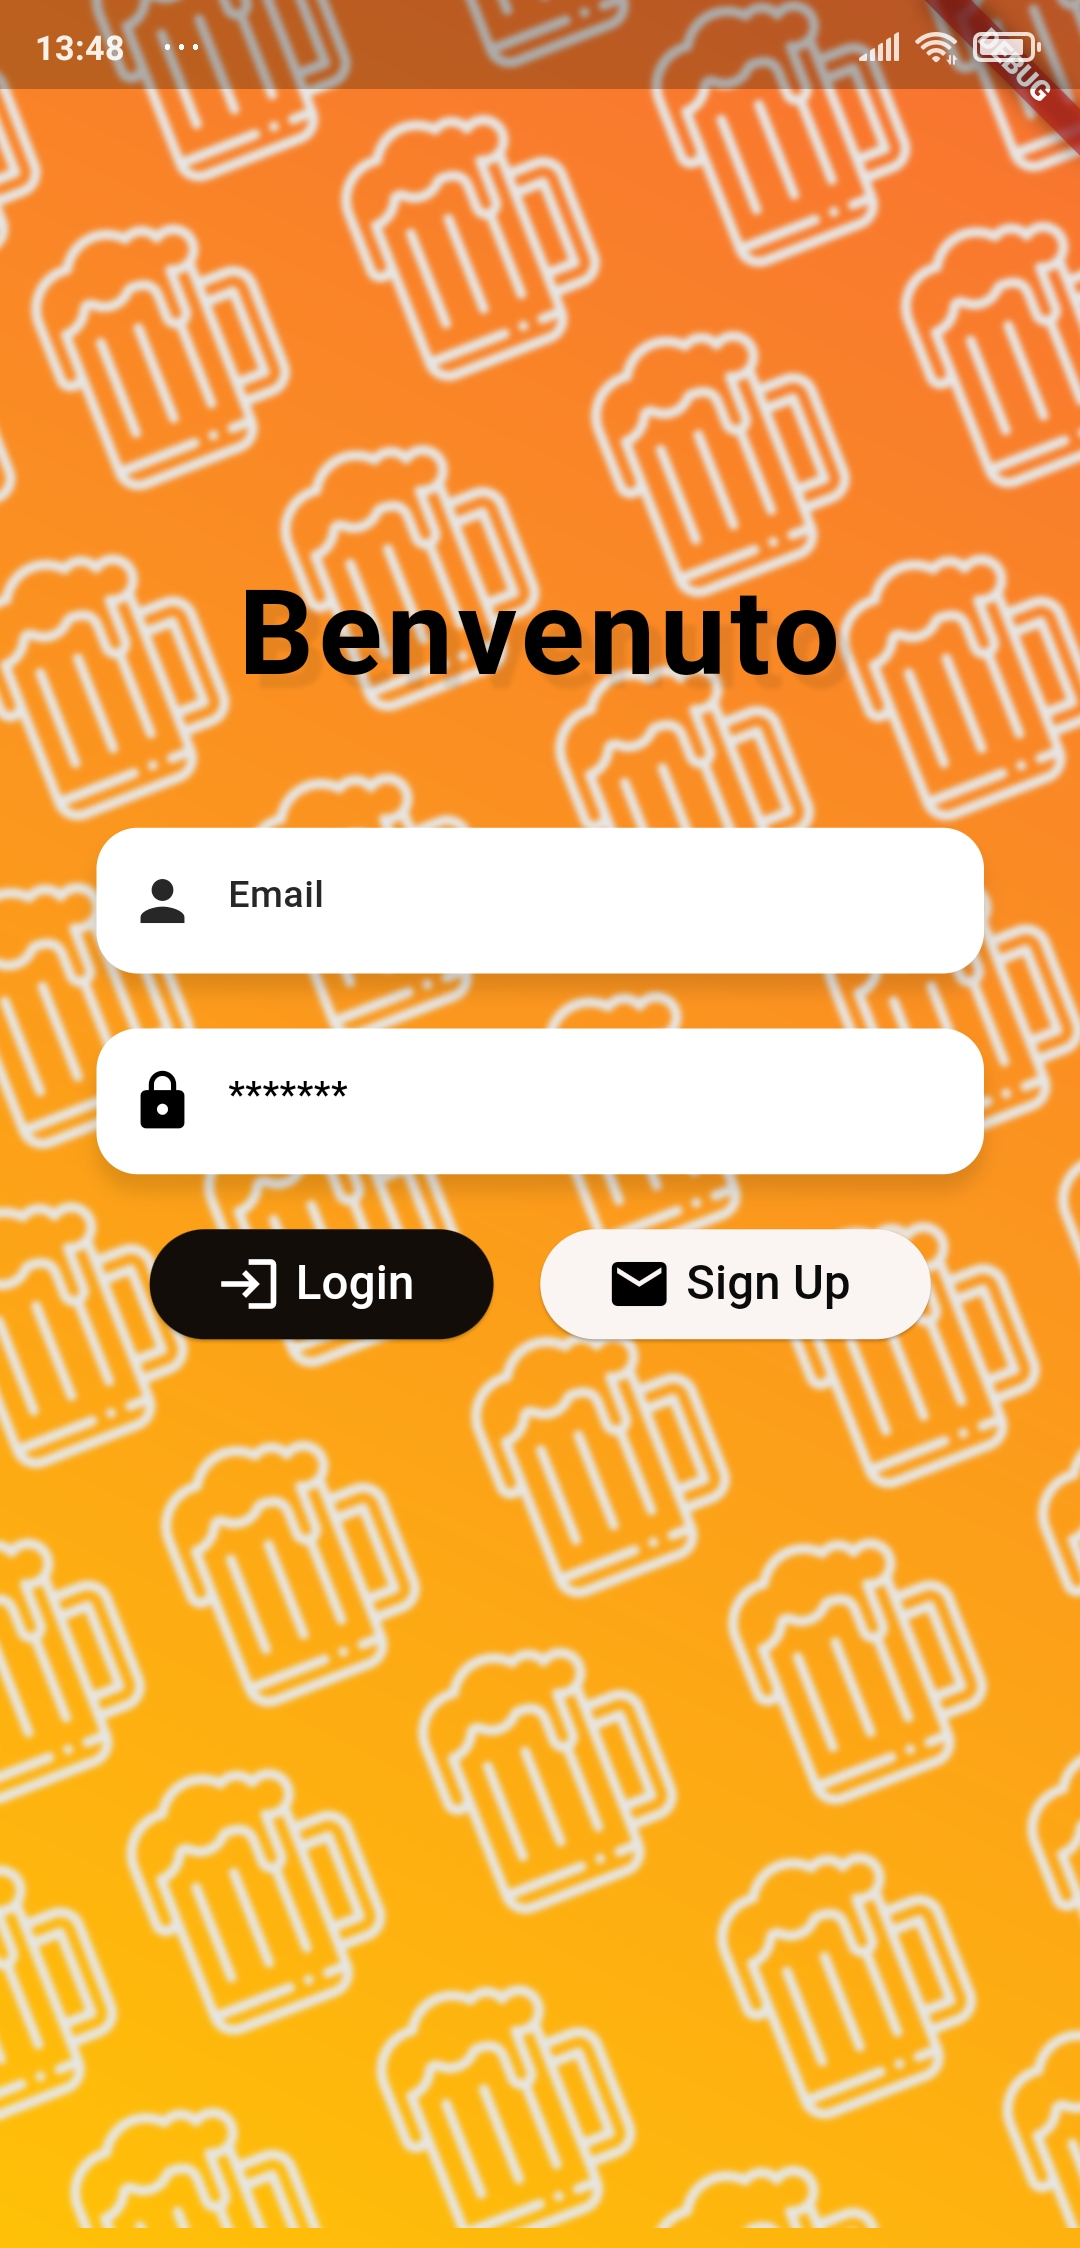
\includegraphics[scale=0.25]{/app_screens/login} % first 
	\space\space\space\space
	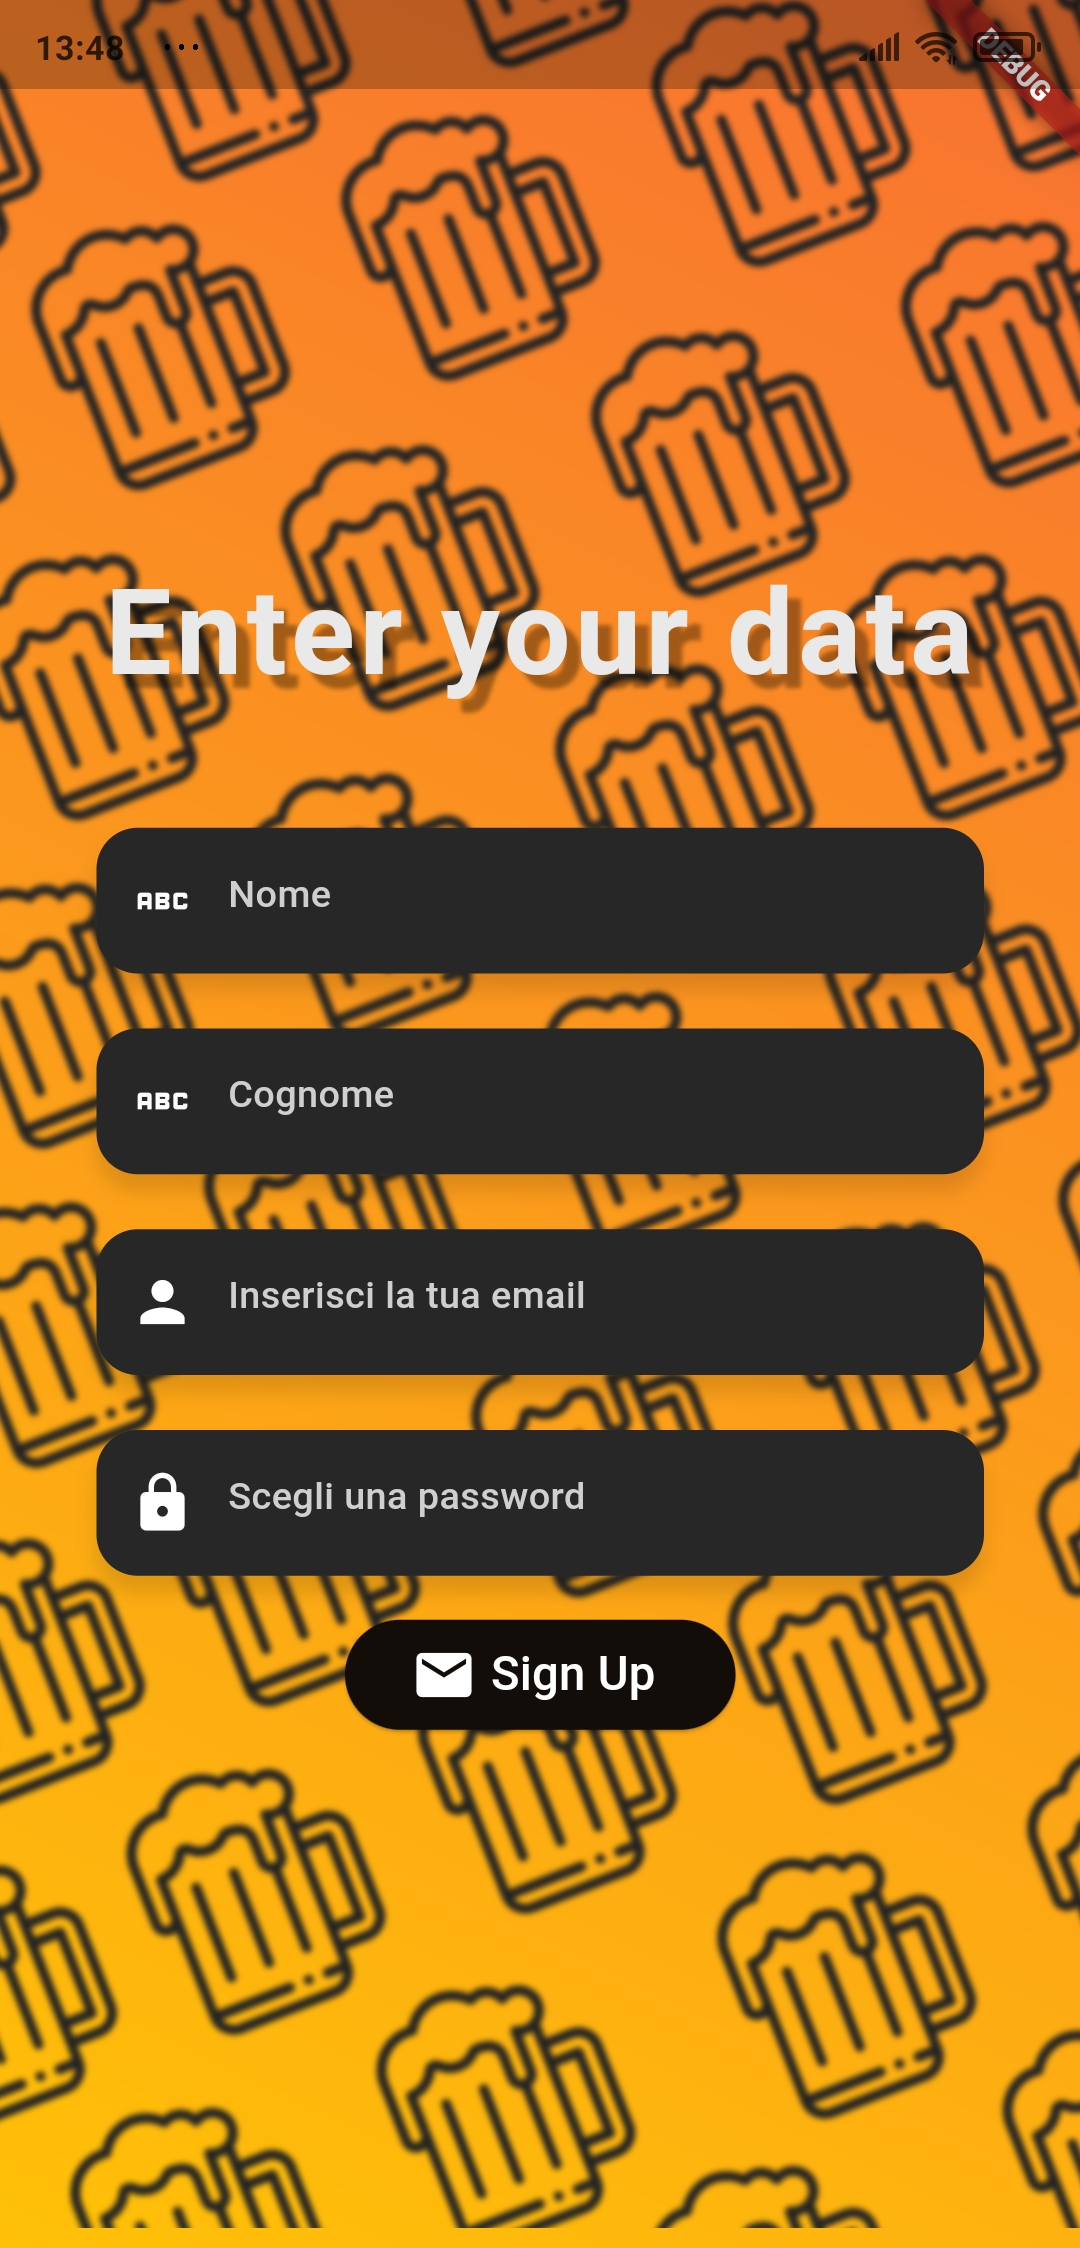
\includegraphics[scale=0.25]{/app_screens/register} % second 
	\caption{The \emph{Login} and \emph{Registration} screens of the app.}
	\label{fig:app1}
	
\end{figure}


After a successful login, the user is presented with their information displayed on different pages. These three pages are actually a single object, created with the \emph{TabBar} class to provide a widget that will slide horizontally among them. The central view gives a welcome to the user and provides direction on what to expect on the side pages. On the left, a quick list of the user's orders, which displays the price and timestamp of each one. On the right page, there is a widget that displays the total amount of money due to the system, and provides a prompt to pay the debt via electronic payment.


\begin{figure}[h!]

		\centering
		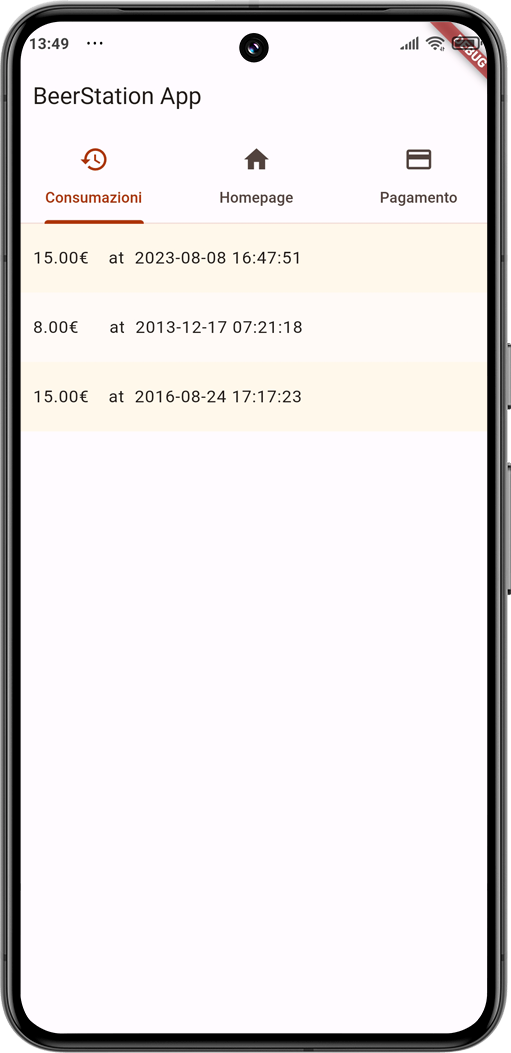
\includegraphics[scale=0.25]{/app_screens/tab} % first 
		\space\space\space
		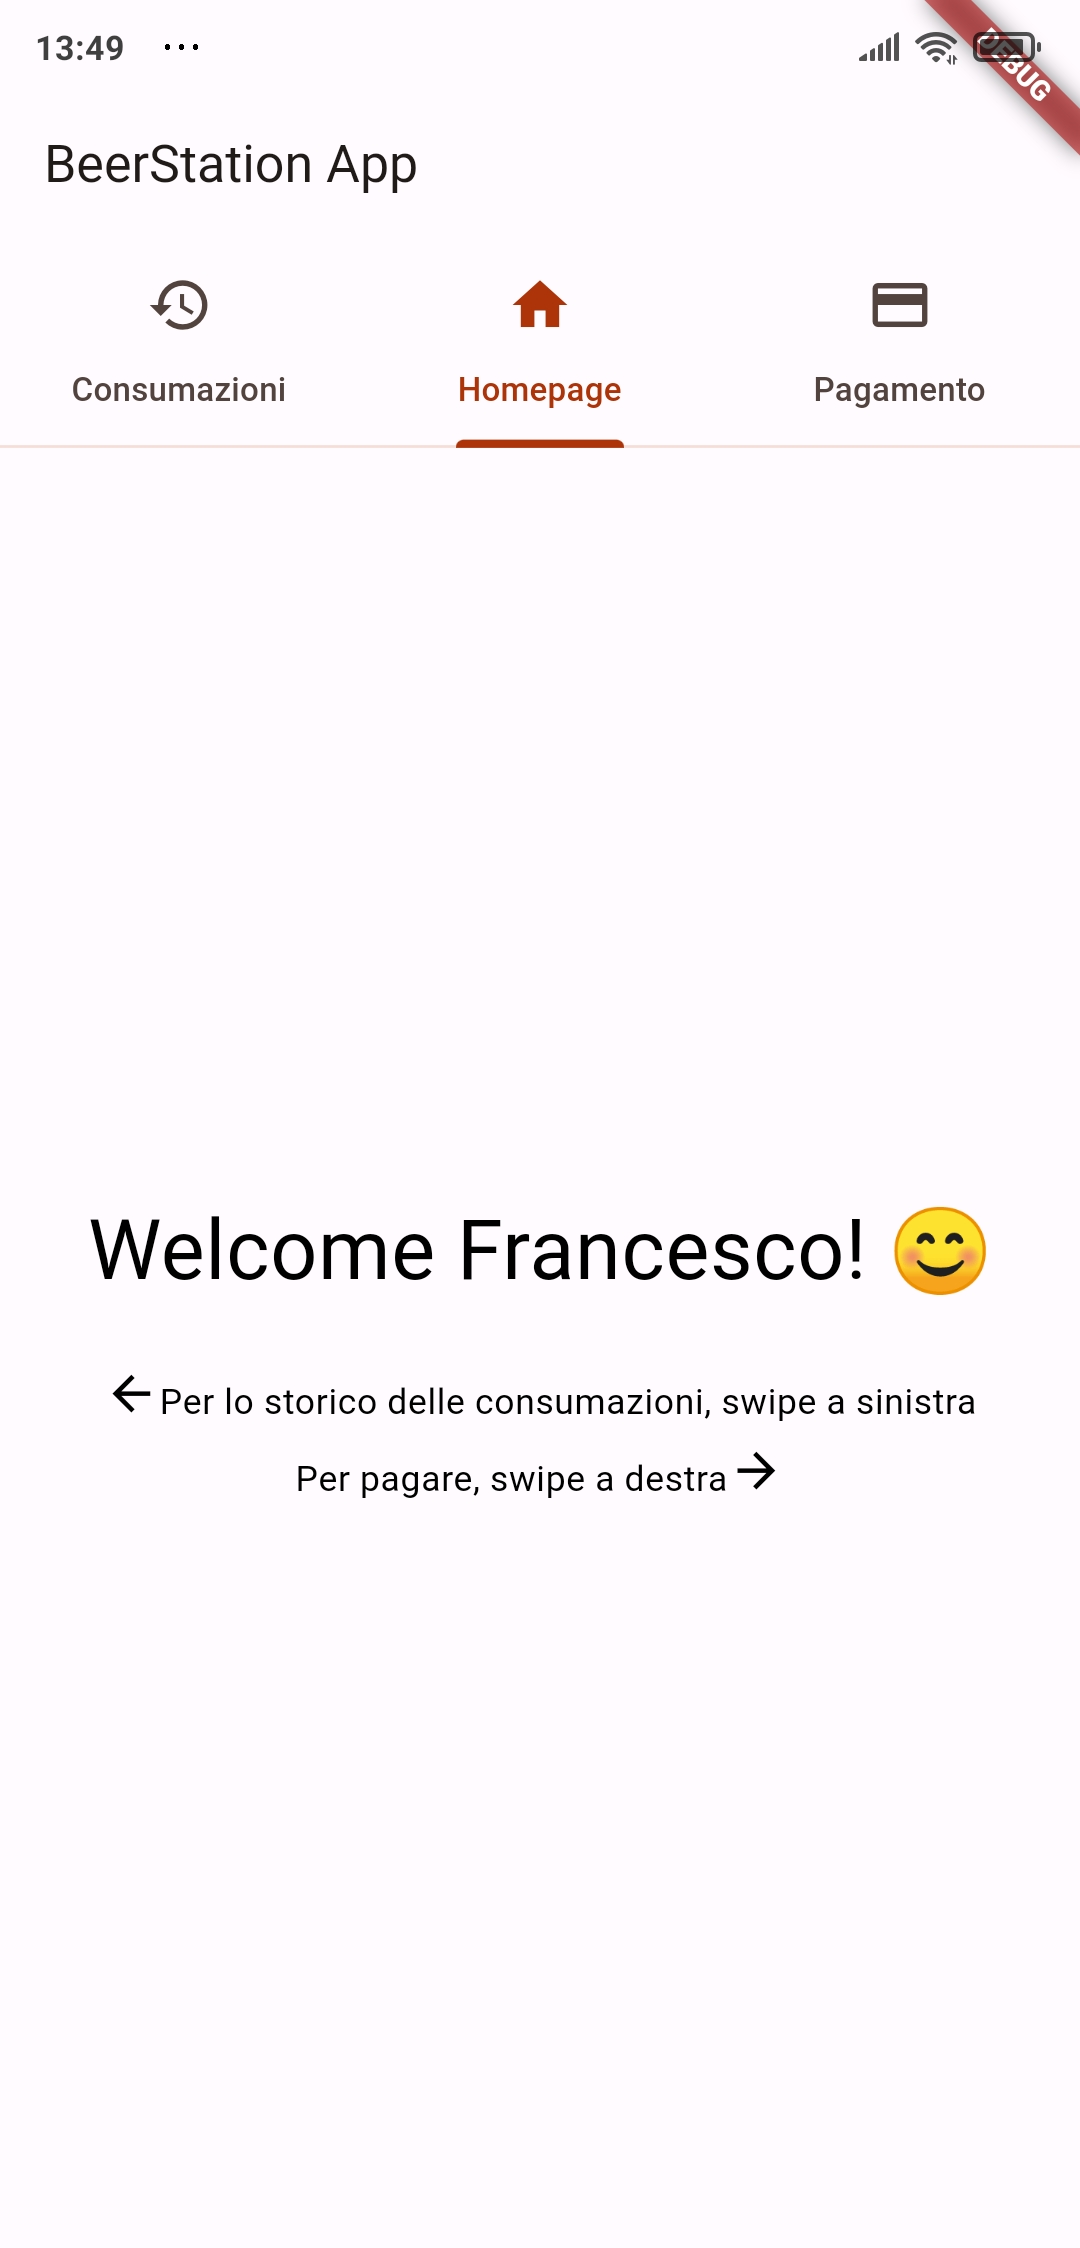
\includegraphics[scale=0.25]{/app_screens/home} % second 
		\space\space\space
		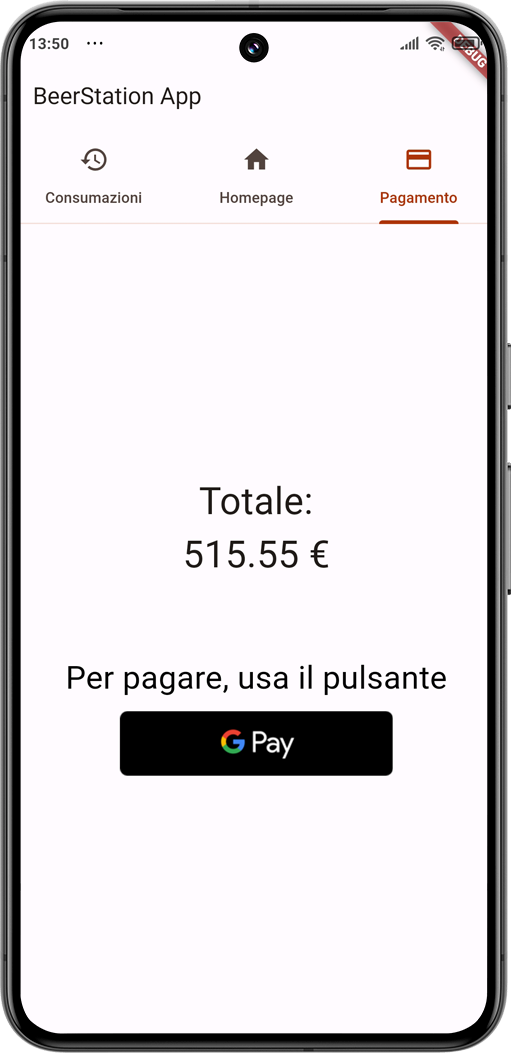
\includegraphics[scale=0.25]{/app_screens/pay} % second 
		\caption{The \emph{History}, \emph{Home} and \emph{Payment} screens of the app.}
		\label{fig:app2}

\end{figure}

\section{PHP API}
The applications needs to query and access the database in order to check the credentials of the users and to obtain data about their total debt and last beverages consumption.
I've decided to create a simple PHP API that would serve the app's requests and return the desired data.
\begin{figure}[htp]
	\centering
	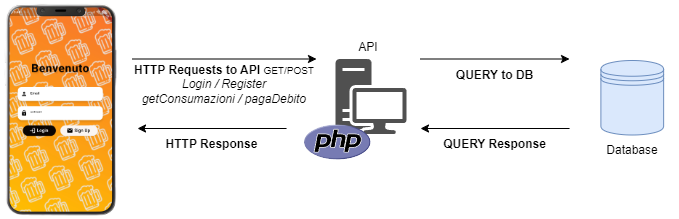
\includegraphics[scale=0.69]{app_diagram} % second 
	\caption{The interaction graph between the app and the server, with the help of a PHP API in the middle.}
	\label{fig:app_diagram}
\end{figure}

Each HTTP request sent from the application is served by the API, which is composed of the following endpoints, each one executing one or more queries to the database server:

\begin{itemize}
	\item \emph{/API/login.php}: Accepts a registered user e-mail and password, and queries the DB for them, returning the user information.
\begin{lstlisting}[language=SQL,style=php_sql]
SELECT * FROM Utente WHERE email='$user_email' AND psw='$user_psw'
\end{lstlisting}
	\item \emph{/API/register.php}: Accepts the data of a new user and tries to  insert them into the database. Upon success, returns the user information.
\begin{lstlisting}[language=SQL,style=php_sql]
INSERT INTO Utente(nome,cognome,email,psw,saldo,data_reg)
VALUES('$user_nome','$user_cognome','$user_email','$user_psw',0,NOW())
\end{lstlisting}
	\item \emph{/API/getConsumazioni.php}: Accepts the id of a registered user, and returns a list of the user's orders.
\begin{lstlisting}[language=SQL,style=php_sql]
SELECT * FROM Consumazione WHERE user_id='$user_id'
\end{lstlisting}
	\item \emph{/API/resetDebt.php}:  Accepts the id of a registered user, and updates the value in the entry, resetting the users debt. Returns the boolean outcome of the request.
\begin{lstlisting}[language=SQL,style=php_sql]
UPDATE Utente SET saldo=0 where id='$user_id'
\end{lstlisting}

\end{itemize}


\chapter{Security}
While working with the technologies discussed in the chapters before, I had to face the topic of security, which is crucial is the IoT field. This field presents a variety of issues, mainly due to the heterogeneity of the thousands of smart-devices and the weak measures adopted by the communication protocol to ensure data protection. In general, the lack of standardized security practices are source of threats for the user data.

In my project, the system works fine, but most of the data stored or transmitted is in plain sight. This chapter will go through the security flaws that were discovered during the development, and for each one it will be discussed the process and procedures used to work around these problems and ultimately solve them.

\section{Access to NFC devices memory}
Starting from the NFC devices, the biggest flaw these types of tags and cards I've used have, is the possibility to tamper with their memory. In fact, depending on the type of support, there is a different level of threat, but in general the main problem consists in being able to manipulate their internal memory without necessarily needing a specific NFC reader. In fact, a NFC enabled smartphone is enough.

Such vulnerabilities could lead to:
\begin{itemize}
	\item Use the refilling stations with tampered NFC glasses, which could be for example linked to a different user without him being aware of it; it's possible but it requires the knowledge of how the data is structured inside the tags.
	\item Cloning another customer NFC tag, which would be easier in terms of needed knowledge of the data structures.
	\item Tamper or clone an NFC card, allowing to impersonate another customer at the beginning of the process
\end{itemize}

In order to prevent this, it's necessary to restrict non-authorized people from accessing the EEPROM memory chips.\pagebreak

\subsection{NTAG213}
The documentation available on NXP's website \cite{ntag213}, provides the specifics about the implementation of an authentication step to access the data on the tag's memory.


\begin{figure}[h!]
	\centering
	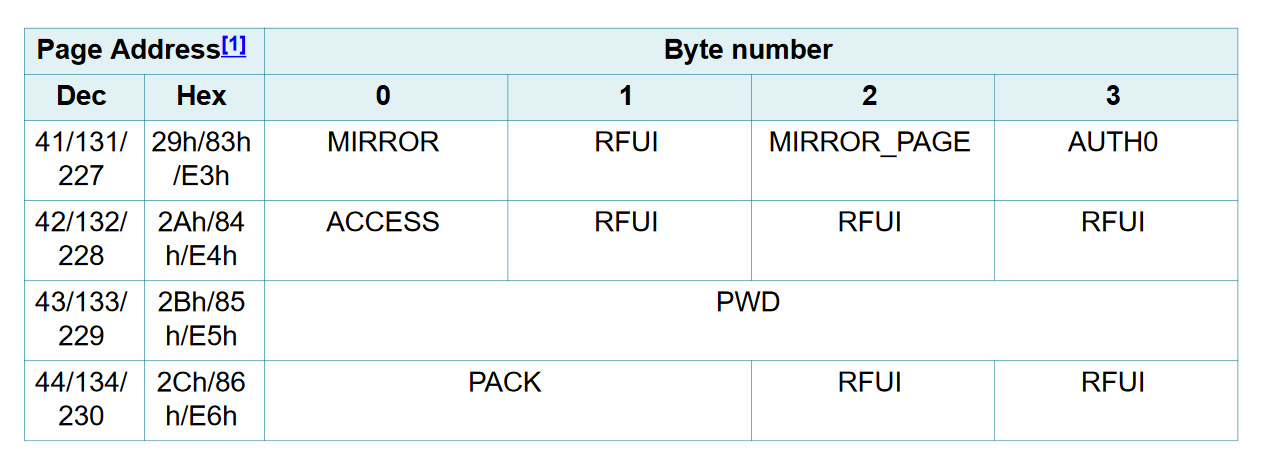
\includegraphics[scale=0.75]{configurationpages}
	\caption{The Configuration Pages, from $0x29$ to $0x2C$ (for NTAG213).}
	\label{fig:configurationpages}
\end{figure}
There are specific pages with fields that are related to the password, access conditions and privileges, which are called \emph{Configuration Pages}:

\begin{itemize}
	\item Page $0x29$ [CFG 0]: Its last byte, the \textbf{AUTH0} byte, indicates the status of the protection of the memory: its value ranges from $0x00$ to $0xFF$, and indicates the first page from which the protection is active:
	\begin{itemize}
		\item $0x00$ means that every page is password protected.
		\item Any value which exceeds the highest page number of the tag (or more generally $0xFF$), means that no page is password protected.
	\end{itemize}
	\item Page $0x2A$ [CFG 1]: Its first byte, the \textbf{ACCESS} byte hosts a configuration in its bits: the last bit, called PROT bit, defines the type of memory protection:
	\begin{itemize}
		\item 0 : Write access is protected by password
		\item 1 : Read and Write access are protected by password
	\end{itemize}
	By default, the ACCESS byte is $0x00$ $\rightarrow$ $(00000000)_2$, PROT = 0.
	\item Page $0x2B$ : Contains a 4 byte password.
	\item Page $0x2C$ : Its first half is occupied by the PACK bytes, which is the value returned after a successful authentication.
\end{itemize}
\newpage
The steps to write the password '1234' $\rightarrow$ $(0x31\ 0x32\ 0x33\ 0x34)_{16}$ on the page $0x2B$, granting read and write protection:
\begin{lstlisting}[language=c++, style=cpp]
	
	// Write PACK buffer on 0x2C
	uint8_t PACKAddress = 0x2C;
	byte PACKbuffer[] = {0xAA, 0xAA, 0x00, 0x00};
	byte PACKSsize = sizeof(PACKbuffer);
	
	status = (MFRC522::StatusCode)mfrc522.MIFARE_Ultralight_Write(
		PACKAddress, &PACKbuffer[0], 4);
	if(status != MFRC522::STATUS_OK){ return; }
	
	// Write the password on 0x2B
	byte PSWbuffer[6]; 
	byte PSWsize = sizeof(PSWbuffer);
	memcpy(PSWbuffer, "1234", 4);
	
	status = (MFRC522::StatusCode)mfrc522.MIFARE_Ultralight_Write(
		PSWAddress, &PSWbuffer[0], 4);
	if(status != MFRC522::STATUS_OK){ return; }
	
	// Write AUTH0 on 0x29
	// By default MIRROR, MIRROR_PAGE = 0x04, 0x00
	uint8_t AUTH0Address = 0x29;
	// In this case from page 04 since I wrote data at that address
	byte AUTH0buffer[4] = { 0x04, 0x00, 0x00, 0x04 };
	byte AUTH0size = sizeof(AUTH0buffer);
	
	status = (MFRC522::StatusCode)mfrc522.MIFARE_Ultralight_Write(
		AUTH0Address, &AUTH0buffer[0], 4);
	if(status != MFRC522::STATUS_OK){ return; }
	
	// Write ACCESS on 0x2A
	uint8_t ACCESSAddress = 0x2A;
	// ACCESS = (10000000) = 0x80 for R/W protection
	byte ACCESSbuffer[4] = { 0x80, 0x00, 0x00, 0x00 };
	byte ACCESSSsize = sizeof(ACCESSbuffer);
	status = (MFRC522::StatusCode)mfrc522.MIFARE_Ultralight_Write(
		ACCESSAddress, &ACCESSbuffer[0], 4);	
\end{lstlisting}
\newpage
A short test to check if the authentication is required for memory writing:
\begin{lstlisting}[language=c++,style=cpp]
	
	// Write test with and without authentication
	uint8_t messageAddress = 0x0A;
	byte message[4] = { 0xAA, 0xAA, 0xAA, 0xAA }; // Test buffer
	byte messagesize = sizeof(message);
	
	Serial.println("Writing (AA AA AA AA) at 0x0A\nWithout authentication...");
	status = (MFRC522::StatusCode)mfrc522.MIFARE_Ultralight_Write(
	messageAddress, &message[0], 4);
	Serial.println(status == MFRC522::STATUS_OK ? "Success" : "Failed");
	
	Serial.println("With authentication...");
	byte PSWBuff[] = { 0x31, 0x32, 0x33, 0x34 };
	authStatus = (MFRC522::StatusCode)mfrc522.PCD_NTAG216_AUTH(&PSWBuff[0], pACK);
	if(authStatus == MFRC522::STATUS_OK) {
		status = (MFRC522::StatusCode)mfrc522.MIFARE_Ultralight_Write(
			messageAddress, &message[0], 4);
			Serial.println(status == MFRC522::STATUS_OK ? "Success" : "Failed");	
	} else {Serial.println( "Auth Failed"); }
\end{lstlisting}
Output:
\begin{lstlisting}[language=c++,style=output]
>> Writing (AA AA AA AA) at 0x0A
>> Without authentication...
>> Failed
>> With authentication...
>> Authenticated
>> Success
\end{lstlisting}

\thinspace

\subsection{MIFARE 1K}
Like the NTAG213, Mifare Classic also offers an authentication process \cite{mifare1k}. Each sector is individually protected, so it's possible to either restrict the access to only a portion of the memory, or to the whole memory.
The Sector Trailer Block in each sector, contains the Keys A and B, and the Access Bits which represent the configuration of the permissions for the sector.

\begin{figure}[h!]
	\centering
	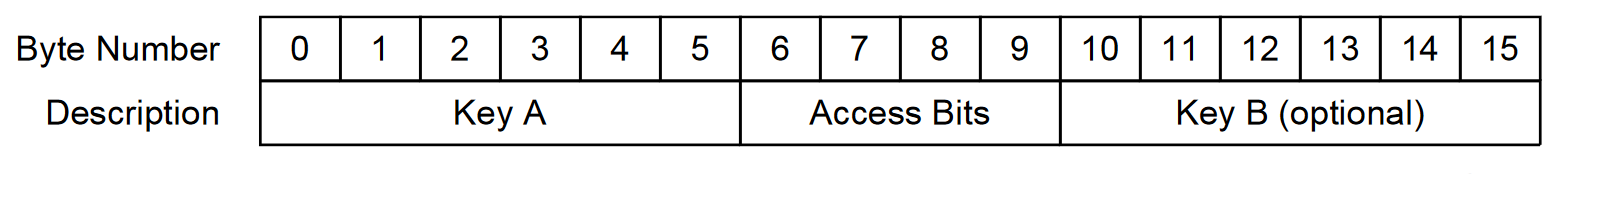
\includegraphics[scale=0.6]{sectortrailerblock} % second 
	\caption{The data organization in the Sector Trailer Block.}
	\label{fig:sectortrailerblock}
\end{figure}
\newpage

Before any memory operation, the card needs to be selected by the PCD and authenticated. Depending on the type of operation and the current configuration of the Access Bits, Key A or B will be needed for the process.
Since every sector trailer has by default the same configuration, 
\begin{itemize}
	\item Both Key A and B are $(FF\ FF\ FF\ FF\ FF\ FF)_{16}$.
	\item Access Bits are $(FF\ 07\ 80)_{16}$.
\end{itemize}
the Secret Keys must be changed, but first it's essential to understand how the Access Bits work.
\thinspace

\subsubsection{Access Bits}
The Access Bits are a configuration represented by the bytes 6, 7 and 8 (the byte 9 can be used as user memory) in every Sector Trailer Block, which is more easy to understand after each byte is converted in its binary equivalent. Each block's access conditions are defined by 3 bits $C1_n, C2_n, C3_n$, with $n$ representing the block's number (0-3).
\begin{figure}[h!]
	\centering
	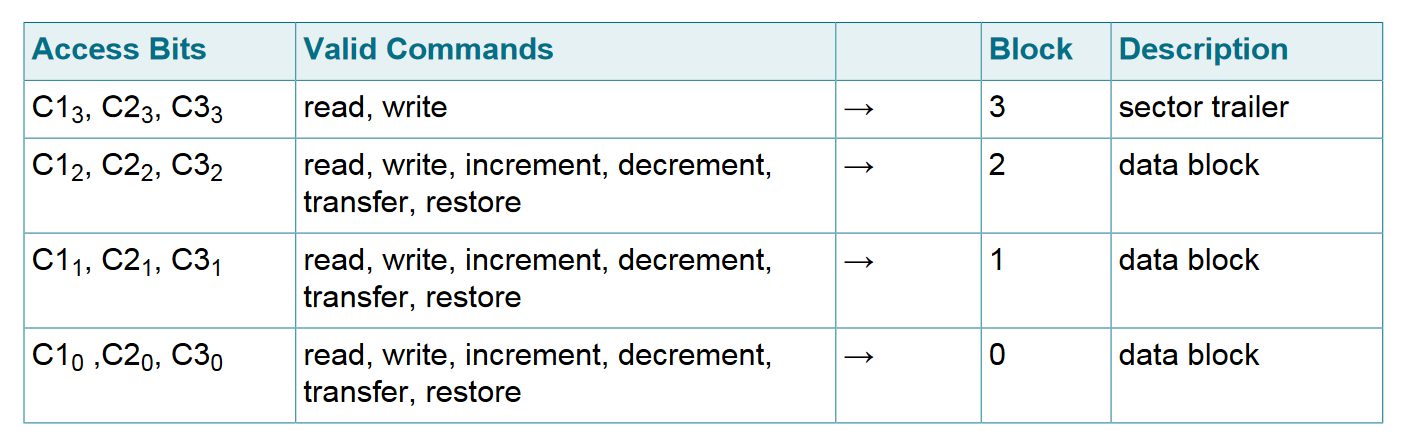
\includegraphics[scale=0.65]{accessconditions} % second 
	\caption{Each block's access conditions, defined by a 3-bits configuration.}
	\label{fig:accessconditions}
\end{figure}

So, each triplet of bits allows \emph{certain} types of operations on the block.\par

These bits are stored both in normal and inverted form for redundancy inside the 3 bytes like this: 

\begin{figure}
	\centering
	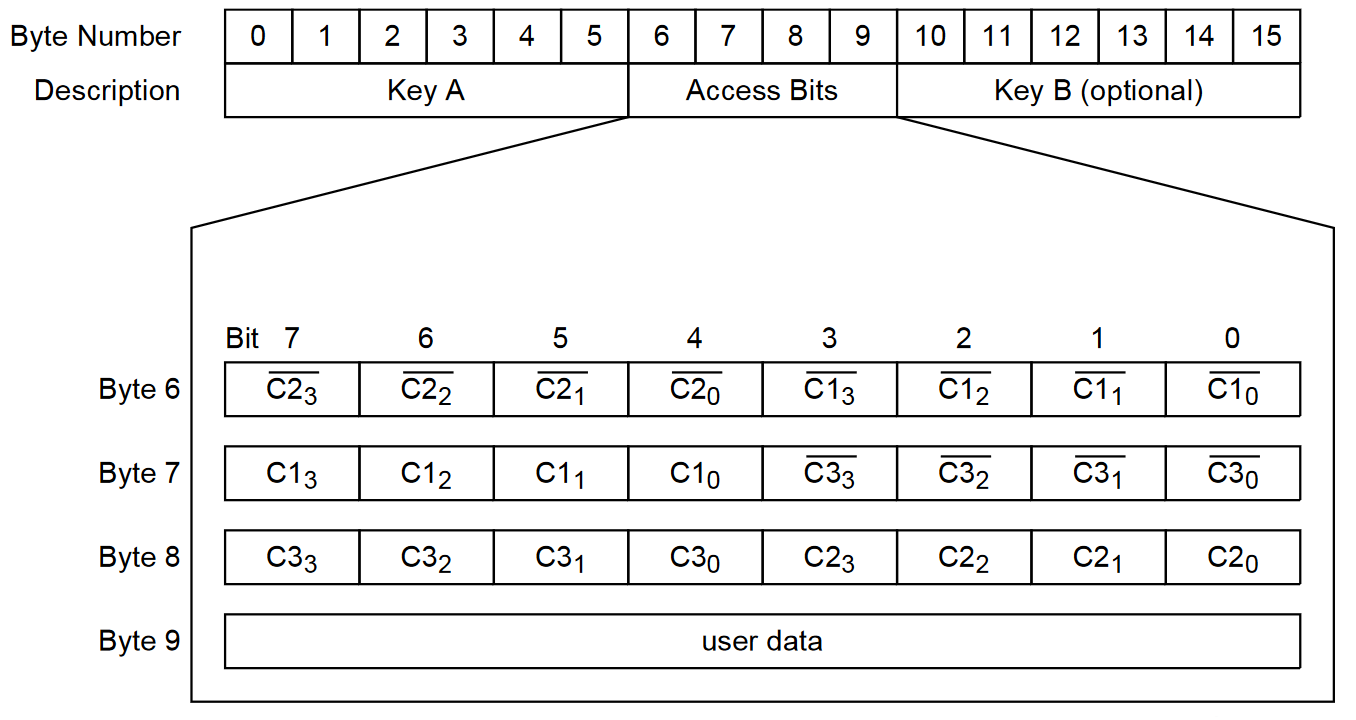
\includegraphics[scale=0.5]{accessconditions2} % second 
	\caption{The bits, both in normal an inverted form.}
	\label{fig:accessconditions2}
\end{figure}

Since the initial configuration of the Access Bits is $(FF\ 07\ 80)_{16}$, in binary is
\[
\begin{array}{ccc}
	(FF)_{16} & \rightarrow  & (11111111)_{2} \\
	(07)_{16} & \rightarrow  & (00000111)_{2} \\
	(80)_{16} & \rightarrow  & (10000000)_{2} \\
\end{array}
\]

From this output, it's possible to deduce that:
\begin{itemize}
	\item The bits $C1_3, C2_3, C3_3$ representing the access conditions for the Sector Trailer Block, are $(0, 0, 1)_2$.
	\begin{figure}[h]
		\centering
		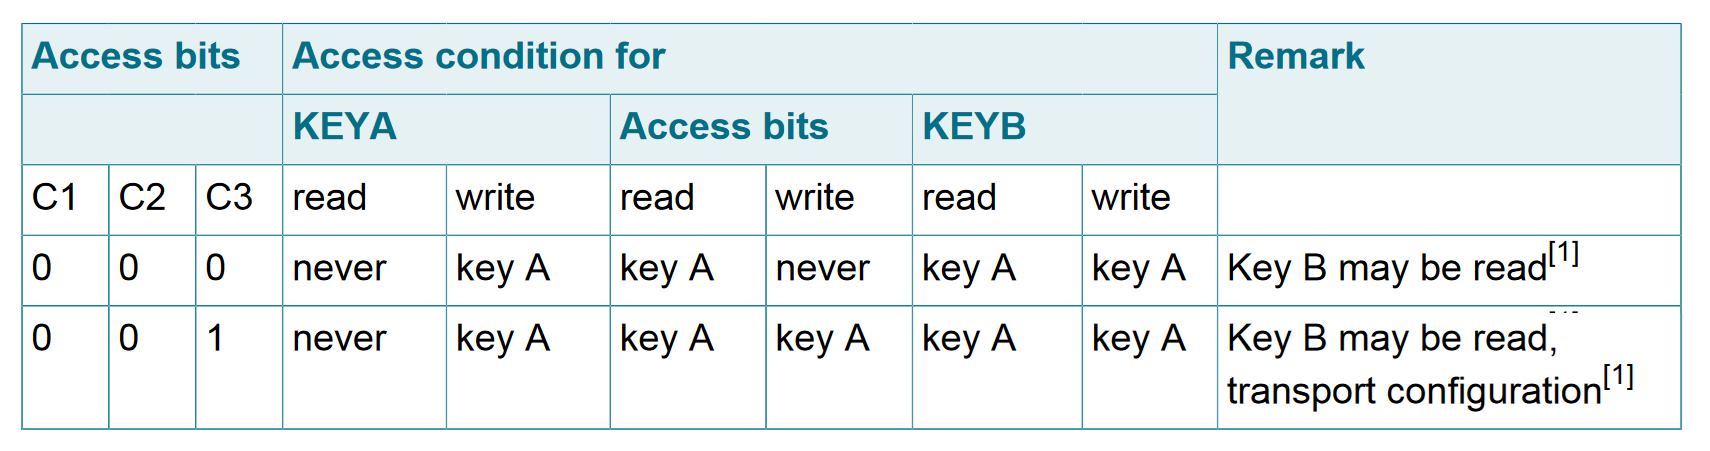
\includegraphics[scale=0.5]{sectortrailerblockconfigurations} % second 
		\caption{The table for the configuration bits of the Sector Trailer.}
		\label{fig:sectortrailerblockconfigurations}
	\end{figure}
	By checking the referencing table, it can be seen that in order to change the Keys A and B, it's necessary to provide only the Key A for authentication.\\
	Note: The "never" entries in the \emph{read KEY A} column will result any attempt to read that memory area to return $(00\ 00\ 00\ 00\ 00\ 00)_{16}$.
	
	\item The other user data blocks have the same configuration $(0, 0, 0)_2$. According to the referencing table, either the Key A or B are needed to read/write the data blocks.
		\begin{figure}[h!]
		\centering
		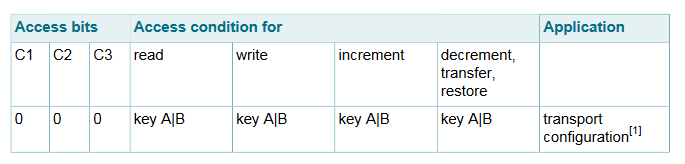
\includegraphics[scale=0.8]{blockconfigurations} % second 
		\caption{The table for the configuration bits of a data block.}
		\label{fig:blockconfigurations}
		\end{figure}
\end{itemize}

Now, all that's left is to authorize the access to the block using the old default Key A and replace both Key A and B with $(AA\ FF\ AA\ FF\ AA\ FF)_{16}$, which will prevent all of the attempts to read the memory using the default keys.
\begin{lstlisting}[ language=c++,style=cpp,caption={The process of changing Keys A and B.},escapeinside=``]
	MFRC522::MIFARE_Key key;
	byte trailerBlockAddr = 7;
	byte buffer[18]; 	// 16 bytes + 2 for CRC
	byte = sizeof(buffer);
	byte dataBlock[] = { //(AA FF AA FF AA FF | FF 07 80 FF | AA FF AA FF AA FF)
		0xAA, 0xFF, 0xAA, 0xFF, 0xAA, 0xFF,	0xFF, 0x07, 0x80, 0xFF, 
		0xAA, 0xFF, 0xAA, 0xFF, 0xAA, 0xFF};
	`\newpage`
	...
	
	for (byte i = 0; i < 6; i++) { key.keyByte[i] = 0xFF; } //Using the default key
	
	// Auth with key A
	Serial.println("Authenticating using key A...");
	status = (MFRC522::StatusCode)mfrc522.PCD_Authenticate(
		MFRC522::PICC_CMD_MF_AUTH_KEY_A, trailerBlockAddr, &key, &(mfrc522.uid));
	if (status != MFRC522::STATUS_OK) {	return; }
	
	// Read Sector Trailer Block 
	status = (MFRC522::StatusCode)mfrc522.MIFARE_Read(trailerBlockAddr, buffer, &size);
	if (status != MFRC522::STATUS_OK) {
		Serial.println("Read failed: " + mfrc522.GetStatusCodeName(status));
	} else { Serial.print("Data in block 7: ");	dump_byte_array(buffer,16);}
		
	// Write Sector Trailer Block
	Serial.println("Writing Sector Trailer Block...")
	status = (MFRC522::StatusCode)mfrc522.MIFARE_Write(trailerBlockAddr, dataBlock, 16);
	if (status != MFRC522::STATUS_OK) {return;}
	
	// Read again Sector Trailer Block
	status = (MFRC522::StatusCode)mfrc522.MIFARE_Read(trailerBlockAddr, buffer, &size);
	if (status != MFRC522::STATUS_OK) {
		Serial.println("Read failed: " + mfrc522.GetStatusCodeName(status));
	} else { Serial.print("Data in block 7: ");	dump_byte_array(buffer,16);}
	
	//Trying to authenticate with the old default key
	status = (MFRC522::StatusCode)mfrc522.PCD_Authenticate(
		MFRC522::PICC_CMD_MF_AUTH_KEY_B, trailerBlockAddr, &key, &(mfrc522.uid));
	if (status != MFRC522::STATUS_OK) {Serial.println("Failed");}
\end{lstlisting}
Output:
\begin{lstlisting}[language=c++,style=output]
	>> Authenticating using key A...
	>> Data in block 7: 00 00 00 00 00 00  FF 07 80 FF  FF FF FF FF FF FF
	>> Writing Sector Trailer Block...
	>> Data in block 7: 00 00 00 00 00 00  FF 07 80 FF  AA FF AA FF AA FF
	>> Failed
\end{lstlisting}

However, it's important to mention that while this is an effective solution for most of the situations, it is still possible to obtain access to the memory using different tools that exploit the communication between the reader and the memory of the device.
\newpage
\subsection{CUS Card}
As mentioned before, the card used is this project is the same model that is commonly used in a variety of different contexts. One of them is the the sports club at the \emph{Università degli Studi di Udine} where the card given upon joining the club gives access to different facilities, such as the gym.

During the early stages of testing the compatibility of the MFRC522 card reader, I tried to test it with said card, as I previously joined the club.
After discovering that it is fact a MIFARE CLASSIC 1K type of card I noticed that its memory sectors were not secured by any protection.\\
On the club's website \cite{cusUdine}, it is stated that the smart card provided is required to access the fitness gym, as one must go through a turnstile that will check the student's subscription and medical certificate.\\
If one is able to tamper with the card's memory sectors, there is a high chance of changing the card's configuration to freely access said facility without actually meeting the requirements.\\
In fact, as I suspected the memory Keys A and B are both set to their default value $(FF\ FF\ FF\ $ $ FF\ FF\ FF)_{16}$. With the same methods explained in the previous chapters, I was able to easily modify the card's bytes values, but as I don't have access to the data structures used to store the relevant information nor the turnstile to physically run multiple test, I can't verify this theory. Although, given the premises and with the right tools, there is a solid chance to exploit this situation.

\begin{figure}[h!]
\centering

\includegraphics[scale=0.6]{cuscard} 
\caption{Exploit of the CUS card.}
\label{fig:cuscardhack}
\end{figure}


\section{MQTT}

MQTT is a convenient and versatile protocol that allows to easily publish and receive messages through the network, but if not used correctly, it can be a source of sensitive information leaks and incoherent transmissions.\\
While developing the communication part of the project, the protocol's lack of protection and encryption measures had to be addressed: everything was potentially visible from unwanted peers, and potentially anyone could send messages to the components of the project that were subscribed to a certain topic.
Of course, these flaws are present only when using the protocol in its most simplified version, but nevertheless, leaving things as they were would have led to critical flaws in the project's aspects such confidentiality and integrity.
\newpage

\begin{figure}[h!]
	\centering
	\frame{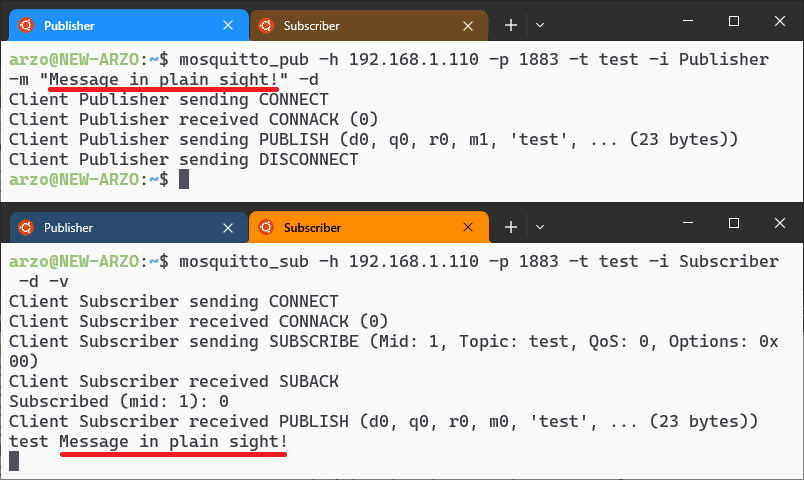
\includegraphics[scale=0.6]{plainsight2}} % second 
	\caption{A simple communication between publisher/subscriber clients.}
	\label{fig:plainsight}
\end{figure}

For instance, with the appropriate tools it is possible to trace and eavesdrop on all the unprotected network traffic of the Local Area Network, gaining access to sensitive information. 
This practice is called \emph{packet sniffing} and allows to inspect the contents of the packet's data like the source and destination address, protocols used, but also the payload that has been transmitted.\\

\begin{figure}[h!]
	\centering
	\frame{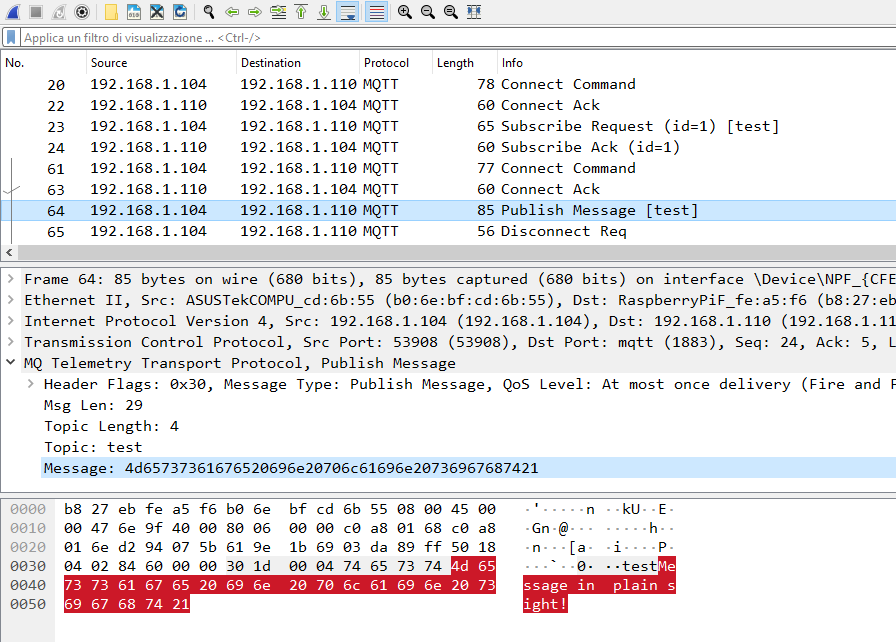
\includegraphics[scale=0.65]{wireshark12}} 
	\caption{A snippet from Wireshark, showing the picked up unprotected data.}
	\label{fig:wireshark1}
\end{figure}
\newpage
An example can be reproduced using \emph{Wireshark} (Fig \ref{fig:wireshark1}), an open source packet analyzer, which can monitor all the MQTT packages (with the proper filter) traveling through the computer's network interface card (which is a restricted case of the attack described before, but this example is an efficient way of demonstrating the vulnerabilities of unprotected communication).
Among all the captured packages, which include the Connection Requests, Connection ACKs, etc... it's possible to see also the message that the Publisher sent to the Broker (and symmetrically the message the broker sent to the Subscriber) and the topic they used,  in plain sight (Fig \ref{fig:plainsight}).

Yet another problem the protocol suffers from, is that if someone discovers the topic name which is used for the communication, then they can also publish messages on that topic to the broker, causing the subscriber clients to receive unwanted messages.\\

When the correct measures are taken, the use of MQTT as the communication protocol is a secure technology.
These two different problems can be solved by  following the principles behind the protocol's security: requiring authentication from every client that connects to the broker and encrypting the connection between the server and each client, using asymmetric encryption.

\subsection{Authentication}
To implement the authentication service in the MQTT protocol, the broker itself first needs to be configured to only accept clients which will authenticate correctly upon connection, and consequently, check if the credentials provided are correct.
The first step is creating a file to store the credentials in the format user:password, which will be also encrypted, using the following command:

\begin{lstlisting}[language=bash,style=bash]
		mosquitto_passwd -c [file_name] [username]
\end{lstlisting}
\begin{figure}[h!]
	\centering
	\frame{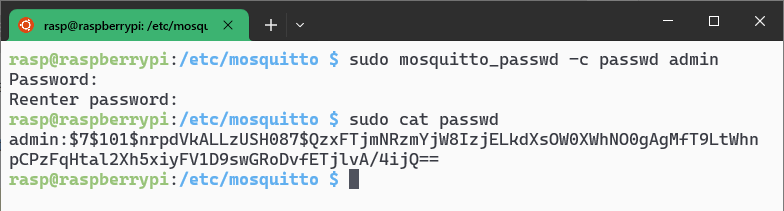
\includegraphics[scale=0.75]{passwd}} % second 
	\caption{The creation of the credentials file.}
	\label{fig:passwd}
\end{figure}

Then, the next step is to add the path to the credential file and the flag to refuse anonymous connections to the mosquitto.conf file:
\begin{lstlisting}[language=bash,style=bash]
		nano /etc/mosquitto/mosquitto.conf
\end{lstlisting}
\begin{figure}[h!]
	\centering
	\frame{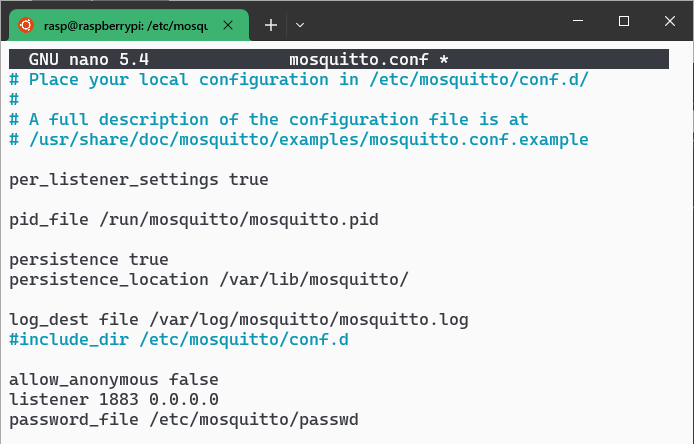
\includegraphics[scale=0.75]{conf1}} % second 
	\caption{The configuration file mosquitto.conf.}
	\label{fig:conf1}
\end{figure}
\newpage

Now, only clients that authenticate themselves can connect and publish/subscribe to topics. If a client tries to connect without authenticating, or using the wrong credentials, the broker will refuse the connection and reply with an appropriate error message. \\
This solves the problem of unwanted clients polluting the topic with their unwanted messages.
\begin{figure}[h!]
	\centering
	\frame{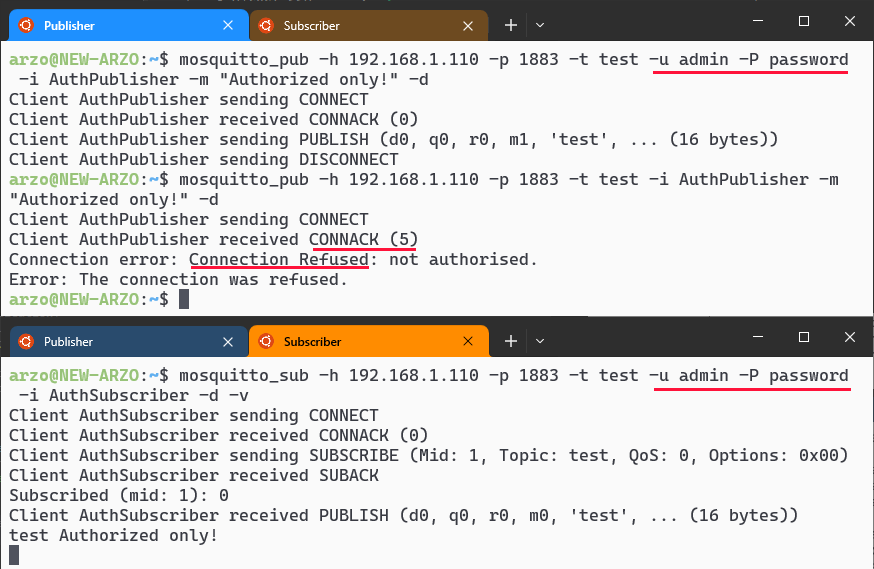
\includegraphics[scale=0.55]{authpubsub}} % second 
	\caption{A communication between authenticated publisher/subscriber clients.}
	\label{fig:authpubsub}
\end{figure}
\newpage
\subsection{TLS/SSL Encryption}
TLS (Transport Layer Security), an improved version of SSL (Secure Socket Layer) is a protocol that ensures a secure communication over the network by encrypting the exchanged data and verifying the authenticity of the connected hosts using certificates.\par
\thinspace

After executing a successful TCP handshake to create a connection between the two hosts, the TLS handshake takes place, and it is in this phase that the client and server (in the project's context, respectively the ESP boards / Python server on one side, and the MQTT broker on the other) set up the secure connection.

During this process, the two sides begin to exchange messages to acknowledge each other, to negotiate on which TLS version the data exchange will happen, to choose which encryption algorithms will be used and lastly to exchange the certificates and keys which will aid to create the secure environment. 

Here, it's possible to see two different types of encryption taking place one after the other: the first, asymmetric, uses a different key on each side, while the symmetric one uses instead the same key on both sides. Respectively, the first one is used during the TLS handshake to set up the connection, while the latter is used once both sides have a shared secret key that allows to encrypt the data sent and decrypt the received messages.

Since the same version of the TLS protocol may not be adopted by the  two devices, they first need to agree on which version will be used. Different versions imply different steps and mechanisms. Both the ESP boards and the Python server's libraries support TLS 1.2, but many utilities are already updated to the newer version, like for example the Linux utility \emph{Mosquitto PubSub}, which I've been using to create the simple instances of Publisher and Subscriber from the bash command line.

The main differences between these two versions are a shorter handshake and removing some encryption algorithms \cite{tlsdifferences} \cite{cloudflaretls}.


\begin{figure}[h!]
	\centering
	\frame{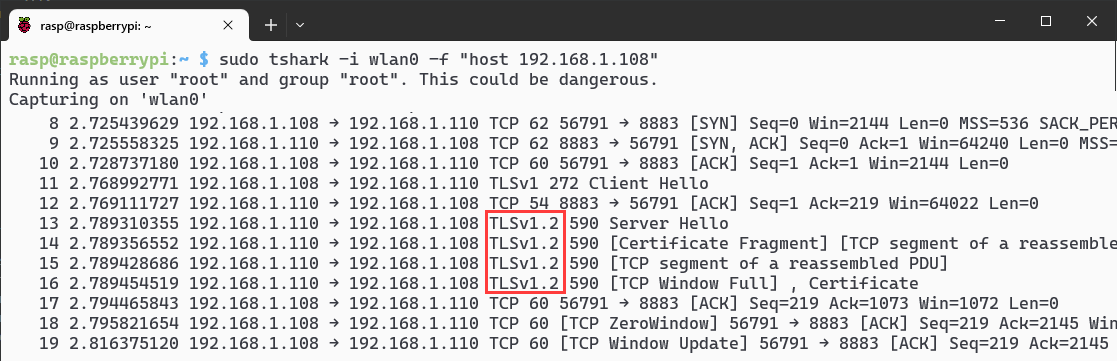
\includegraphics[scale=0.43]{tshark}} % second 
	\caption{Using the utility tshark on the Raspberry, shows that the ESP boards use TLS 1.2.}
	\label{fig:tshark}
\end{figure}

\emph{Note}: I had to use the much lighter utility tshark instead of Wireshark since the Raspberry Pi in my possession is not powerful enough to run the program.
\newpage
\subsubsection{The TLS Handshake}
\begin{figure}[h!]
	\centering
	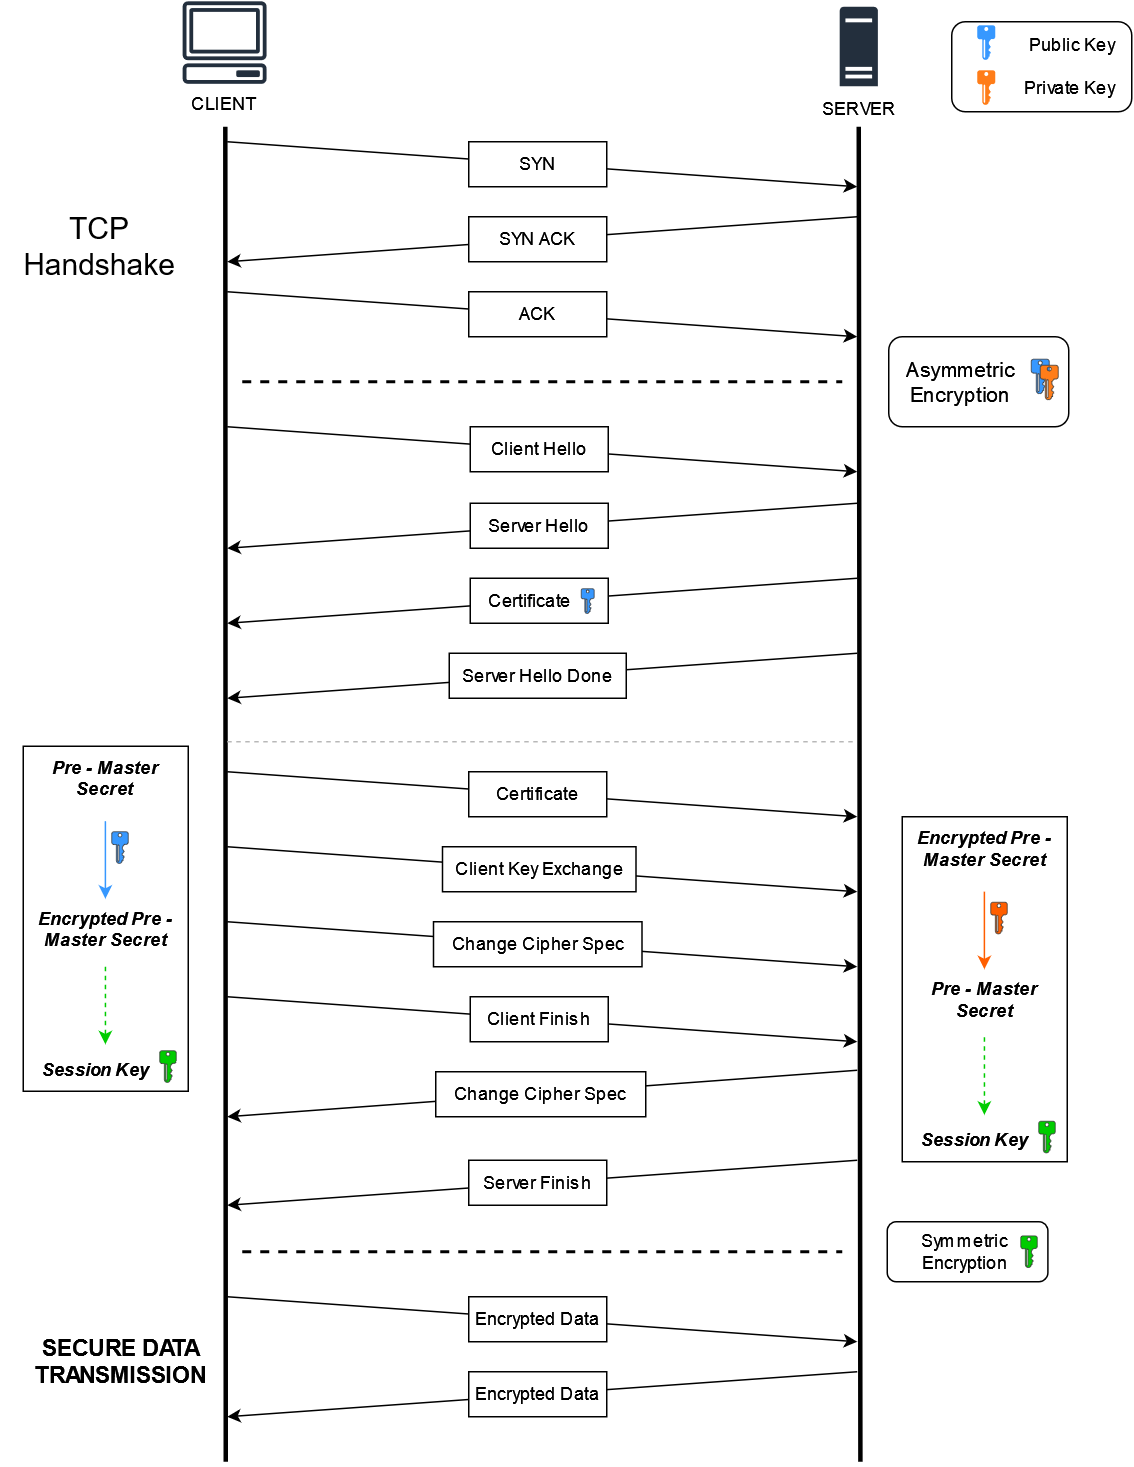
\includegraphics[scale=0.4]{tls_finale} % second 
	\caption{A general view of the TLS 1.2 sequence diagram.}
	\label{fig:tls}
\end{figure}
\newpage
The handshake can be divided in different phases:
\begin{enumerate}
\item The first phase is used to establish security capabilities, such as protocol version, algorithms, cipher suites, Session ID ...

\begin{itemize}
	\item After a TCP connection, the client sends to the server a "\lstinline[style=bash]|Client Hello|" message, which lists all the TLS versions supported by the client, the cipher suites and compression methods available and a random client value.
	\item The server receives the "\lstinline[style=bash]|Client Hello|" and responds with a "\lstinline[style=bash]|Server Hello|" message. In this message, the server will pick the TLS version and the cipher suite from the previous message, and will also send a random server value.
\end{itemize}

\item In the second phase, the server sends more data to the client:

\begin{itemize}
	\item The server sends his certificate to the client for authentication purposes. It also contains the server's Public Key which will be later used.
	\item After potentially requesting the client to provide its certificate, since the server could also want to validate the other side, it sends a "\lstinline[style=bash]|Server Hello Done|" signal, stating the end of the phase.
\end{itemize}

\item The client replies and sends his last messages:

\begin{itemize}
	\item The client sends its certificate to the server.
	\item The client creates a \textbf{Pre-Master Secret} with the two randomly generated values exchanged during the \lstinline[style=]|Client/Server Hello| messages using an algorithm which they agreed upon before (usually RSA). 
	Then it encrypts the value using the server's Public Key, and sends it to the server: now both have the same Pre-Master Secret, since the Server can decrypt the message using its Private Key.\\
	Now both ends can derive the \textbf{Master Secret}, which is used to generate the \textbf{Session Keys} that will allow to have an encrypted conversation. It's important that both sides obtain the same result, as otherwise it is not possible to communicate.
	\item If requested before, the client sends hashed information that the server can use to validate its certificate.
	\item Before sending a "\lstinline[style=bash]|Client Finish|" message, it also sends a "\lstinline[style=bash]|Change Cipher Spec|" that tells the server to start encrypting the conversation.
	\item Lastly, the server also responds with a "\lstinline[style=bash]|Change Cipher Spec|" before concluding the handshake process with a "\lstinline[style=bash]|Client Finish|" message.
\end{itemize}

\item With the handshake concluded, client and server can exchange data over a secure and encrypted connection.

\end{enumerate}
\newpage
In order to implement these practices, the certificates were generated using the OpenSSL package which is the implementation of the SSL open-source protocols \cite{tlsmqtt} \cite{tlsmosquitto}. First, the Certificate Authority certificate is created, allowing to generate later other trusted certificates issued by the CA.

\begin{lstlisting}[language=bash,style=bash]
	# Generating the certificate and key for the CA (Certificate Authority)
	openssl req -new -x509 -days 365 -extensions v3_ca -keyout ca.key -out ca.crt
	>> passphrase : abc123
	>> CN : iotproject
	sudo chmod 644 ca.key
\end{lstlisting}

Then, a set of .crt, .key files are created for every device that needs to safely communicate with the MQTT broker using the CA certificate.

\begin{lstlisting}[language=bash,style=bash]
	# Generating the key, the Certificate Signing Request (.csr) of the Broker
	openssl genrsa -out broker.key 2048
	sudo chmod 644 broker.key
	openssl req -out broker.csr -key broker.key -new
	>> CN : 192.168.1.110 (RPi IP address)
	
	# and then the Broker certificate
	openssl x509 -req -in broker.csr -CA ../ca/ca.crt -CAkey ../ca/ca.key 
		-CAcreateserial -out broker.crt -days 365
	>> passphrase : abc123
	
	# Repeat to create .crt and .key files for ESP boards and Python server
\end{lstlisting}

Editing the mosquitto.conf file \cite{mosquittoconfig}, adding the paths to the files, changing the port to 8883 (commonly used when TLS is implemented) and setting some flags in order to start using certificates:

\begin{figure}[h!]
	\centering
	\frame{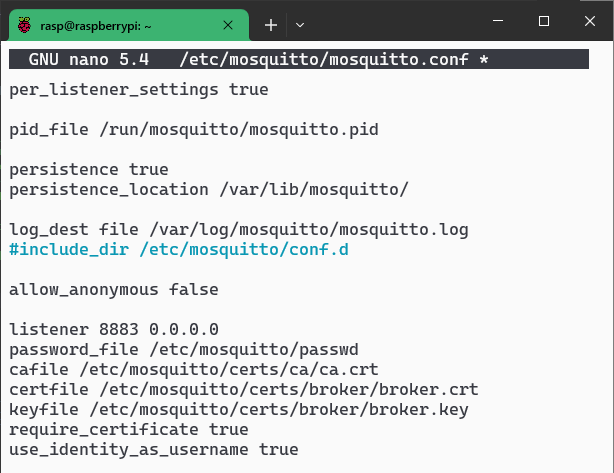
\includegraphics[scale=0.75]{conf2}} % second 
	\caption{The updated version of mosquitto.conf.}
	\label{fig:conf2}
\end{figure}
\newpage

\begin{figure}[h!]
	\centering
	\frame{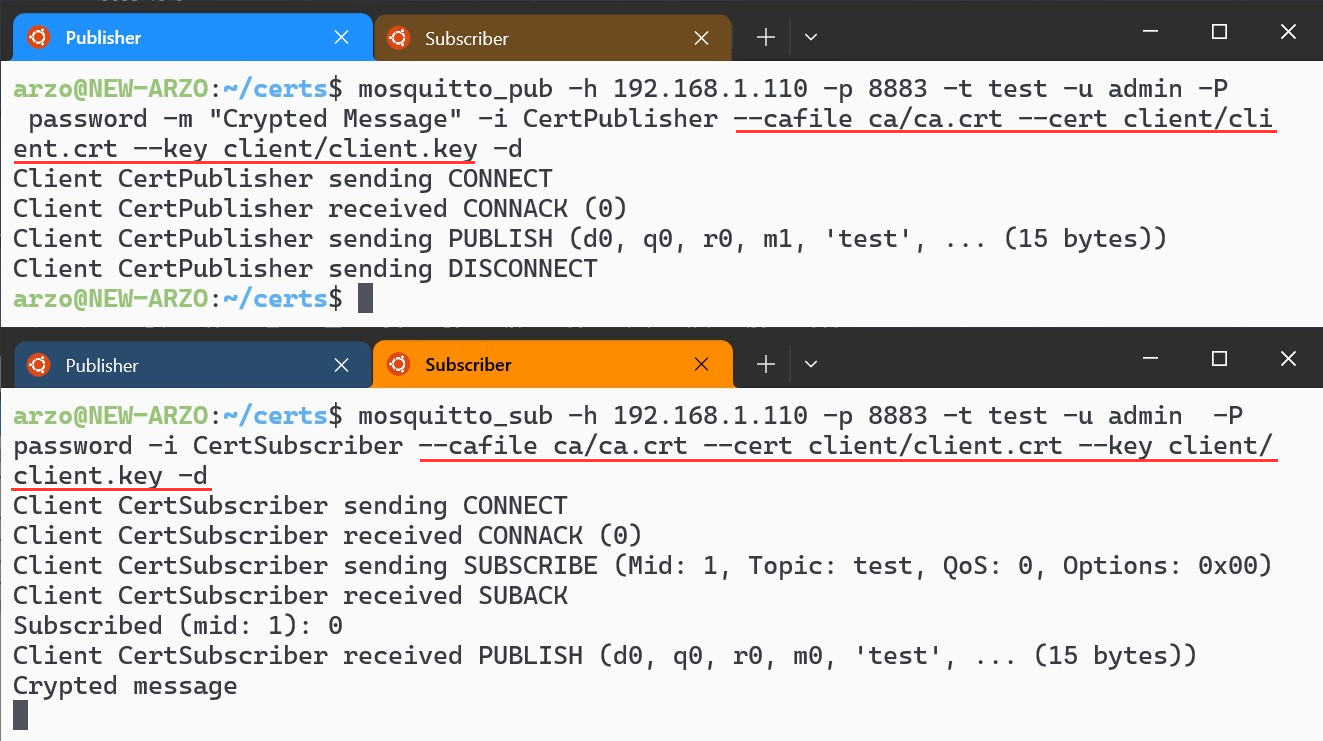
\includegraphics[scale=0.35]{tlspubsub}} % second 
	\caption{A communication example between two clients over TLS using authentication and certificates.}
	\label{fig:tlspubsub}
\end{figure}

Using again Wireshark to capture the packets between the broker and a clients now shows very little information: it is still possible to deduce that the two machines started an TLS handshake and that afterwards there has been a communication, but its contents are not in plain sight like before. Instead, they have been encrypted using the Session Key generated during the handshake.

\begin{figure}[h!]
	\centering
	\frame{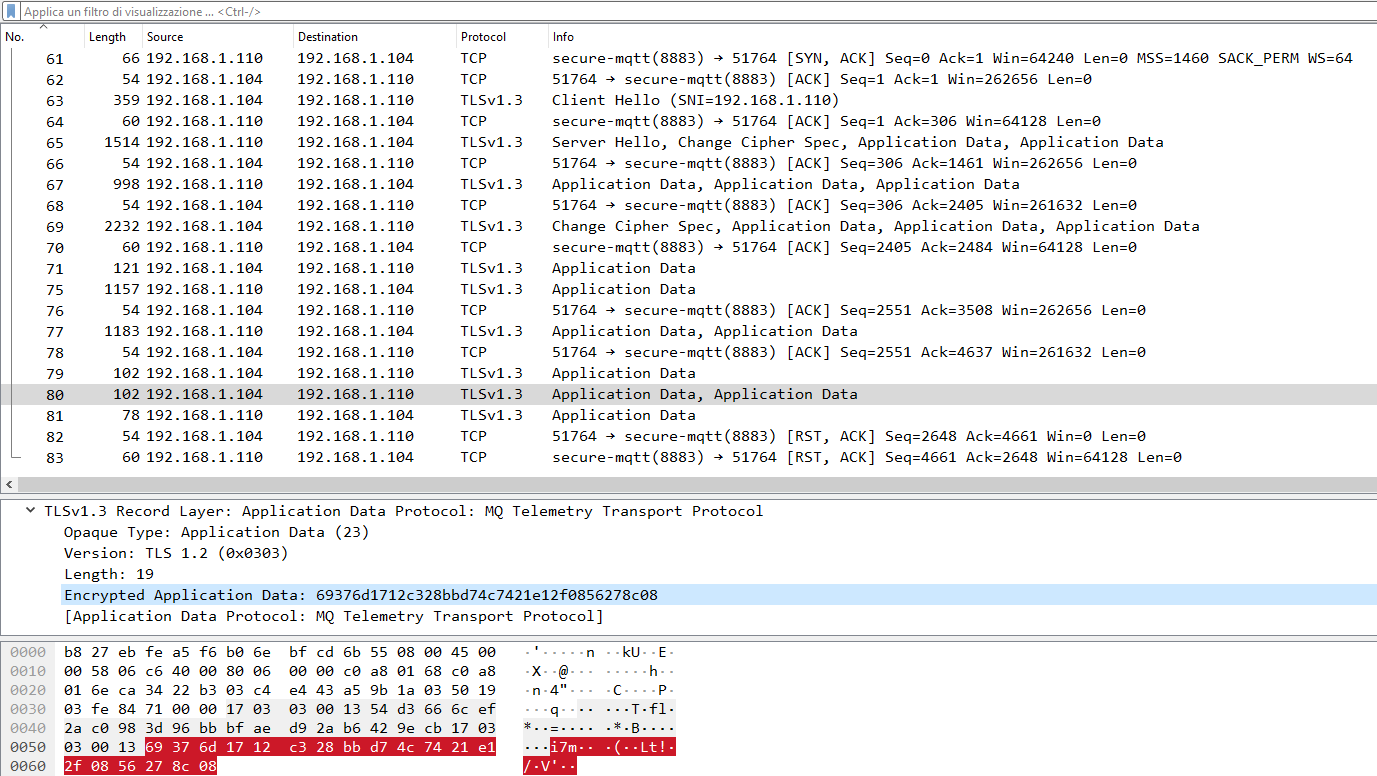
\includegraphics[scale=0.5]{wiresharktls}} % second 
	\caption{The packets are now encrypted, hiding the message sent by the Publisher.}
	\label{fig:wiresharktls}
\end{figure}


Now, to implement TLS on the ESP32/ESP8266 communication with the broker, each certificate/key can be easily printed out and copied from the terminal:

\begin{lstlisting}[language=bash, style=bash]
	
	$ sudo cat certs/ca/ca.crt
	>>	-----BEGIN CERTIFICATE-----
		MIIDnTCCAoWgAwIBAgIUcb6V2nxgsru5LWsgMkslH7WswiowDQYJKoZIhv
		BQAwXjELMAkGA1UEBhMCSVQxDjAMBgNVBAgMBWl0YWx5MRAwDgYDVQQHDA
		c3RlMQ4wDAYDVQQKDAV1bml1ZDENMAsGA1UECwwEZG1pZjEOMAwGA1UEAw
	...
\end{lstlisting}

It is possible to load and use them inside an Arduino sketch thanks to some functions of the ESP8266WiFi library, which are internally provided by the BearSSL library.
\begin{lstlisting}[language=c++,style=cpp]
	
	/*Broker's address as IPAddress class object; 
	 Makes it easier checking the CA certificate*/
	IPAddress broker(192,168,1,110);
	
	const char ca_cert[] PROGMEM = R"EOF(
	MIIDnTCCAoWgAwIBAgIUcb6V2nxgsru5LWsgMkslH7WswiowDQYJKoZIhvcNAQEL
	...	
		)EOF" ;
	const char client_private_key[] PROGMEM = ... ;
	const char client_cert[] PROGMEM = ... ;
	
\end{lstlisting}

\begin{lstlisting}[language=c++,style=cpp]
	
	BearSSL::WiFiClientSecure espClient;
	
	void setup() {
		//Setting up the certificates and key
		BearSSL::X509List *serverTrustedCA = new BearSSL::X509List(ca_cert);
		BearSSL::X509List *serverCertList = new BearSSL::X509List(client_cert);
		BearSSL::PrivateKey *serverPrivKey = new BearSSL::PrivateKey(client_private_key);
		
		espClient.setTrustAnchors(serverTrustedCA);
		espClient.setClientRSACert(serverCertList, serverPrivKey);
		// Required for X.509 validation
		setClock();
		...
	
\end{lstlisting}

As the two ESP boards have different MCU, they work with different libraries, but the concept and the process behind the implementation of TLS on ESP32 is the same.

The two types of ESP board used posses different MCU and thus need different libraries to implement a TLS connection, but the overall differences are limited to a slight difference in the code. The procedure and concepts behind are the same, hence here I'll show only one of the two implementation, the one on the ESP8266.



\newpage
\section{App Requests Encryption}

To establish a secure connection between the Android Application on the smartphone and the API that retrieves and publishes data from the MySQL database, the symmetric encryption mechanism was used to accomplish the goal. Both ends have stored a key which allows to encrypt and decrypt the exchanged data.\\
Using PHP and Flutter support for the Object Oriented Programming paradigm, a class \emph{Encryption} is declared, which is responsible for providing methods to encrypt and decrypt data using the two homonymous classes.\par

In Flutter this is possible with the support of the \emph{encrypt} and \emph{crypto} packages:

\begin{lstlisting}[language=java,style=java]
	
	import 'package:encrypt/encrypt.dart';
	import 'package:encrypt/encrypt.dart' as encryptPackage;
	import 'package:crypto/crypto.dart';
	
	class Encryption {
		static final Encryption instance = Encryption._();
		late IV _iv;
		late Encrypter _encrypter;
		
		Encryption._() {
			final utf8_key = utf8.encode('fh934fhdwofj340rjf390hf390h43232');
			final utf8_iv = utf8.encode('hf934fhewfudsifs');
			
			final key = sha256.convert(utf8_key).toString().substring(0, 32);
			final iv = sha256.convert(utf8_iv).toString().substring(0, 16);
			_iv = IV.fromUtf8(iv);
			_encrypter =
			Encrypter(AES(encryptPackage.Key.fromUtf8(key), mode: AESMode.cbc));
		}
		
		String encrypt(String toEncrypt) {
			return _encrypter.encrypt(toEncrypt, iv: _iv).base64;
		}
		
		String decrypt(String toDecrypt) {
			final coso = Encrypted.fromBase64(toDecrypt);
			return _encrypter.decrypt(coso, iv: _iv);
		}
	}
	
\end{lstlisting}

The Encryption class methods can be used in any other Flutter file after importing the \emph{utils.dart} file by using the syntax:

\begin{lstlisting}[language=java,style=java]
	
	import 'package:drinks/utils.dart';
	String psw = Encryption.instance.encrypt(controllerPassword.text);
	
\end{lstlisting}
\newpage

On the other side of the communication, the \emph{OpenSSL} methods are already imported in the PHP environment, so all is left to do is to create a class with the same goal as before:

\begin{lstlisting}[language=php,style=php]
	
	class Encryption {
		private string $method = 'AES-256-CBC';
		private string $key;
		private string $iv;
		
		public function __construct() {
			$basicKey = 'fh934fhdwofj340rjf390hf390h43232';
			$iv = 'hf934fhewfudsifs';
			
			$this->key = substr(hash('sha256', $basicKey), 0, 32);
			$this->iv = substr(hash('sha256', $iv), 0, 32);
		}
		
		public function encrypt($toEncrypt) {
			return openssl_encrypt($toEncrypt, $this->method, $this->key, 0, $this->iv);
		}
		public function decrypt($toDecrypt) {
			return openssl_decrypt($toDecrypt, $this->method, $this->key, 0, $this->iv);
		}
	}
	
\end{lstlisting}

The class can be instantiated in another PHP file  importing the \emph{utils.php} file, by using the syntax:

\begin{lstlisting}[language=php,style=php]

	$encryption = new Encryption();
	$user_psw = $encryption->decrypt($_POST['psw']);
	 
\end{lstlisting}

By implementing these changes to the code on each end, it was possible to establish a secure data exchange.

\begin{figure}[h]
	\centering
	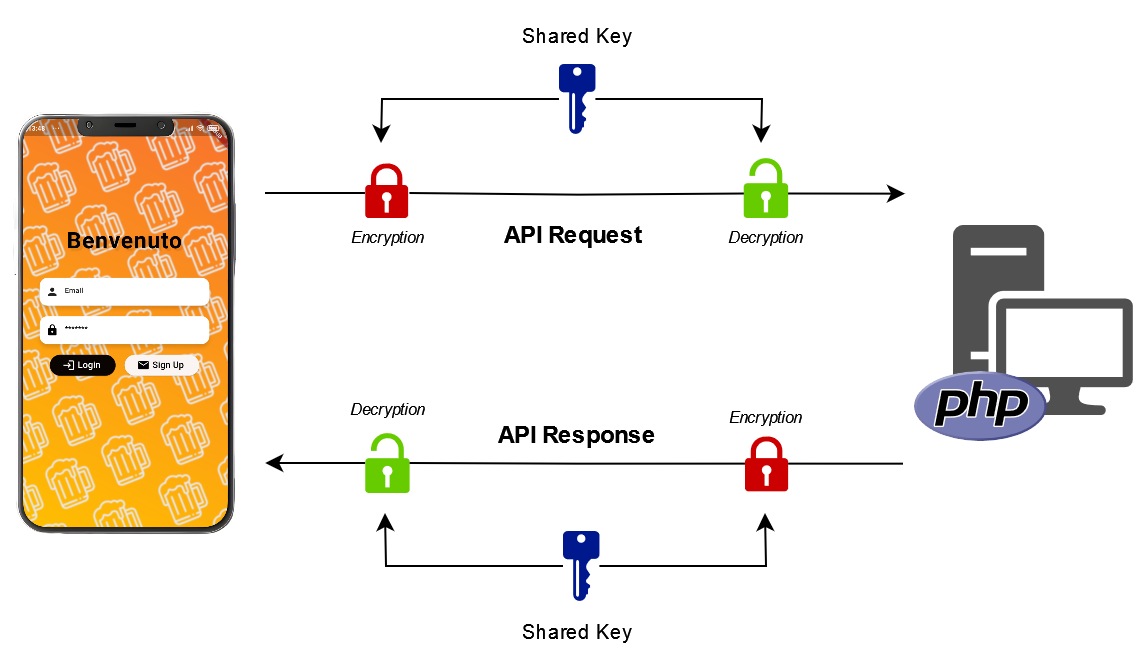
\includegraphics[scale=0.3]{phpapi}
	\caption{The diagram of the now secure data exchange between a mobile client and the PHP API.}
	\label{fig:phpapi}
\end{figure}

\chapter{Considerations and Improvements}
\section{What I've learned}
During the realization of this project, I had the chance to learn a lot of things. It was the first time creating something like this, watching the pieces falling in their places step by step. Every aspect of this work required to pose myself a problem and find a suitable solution, while trying to maintain the balance between compromise and requirements. I was able to work with multiple products and technologies: most of them were already known thanks to the experience during various courses, but I also had to face the challenge of learning how to use and create synergies with other I had never worked with.

The experience in my internship allowed me to learn more and actually implement notions I had learned in the most recent courses, and also to understand how to implement new functionalities on an already existing project that needed to meet new requirements.


\section{Improvements}

This work is the result of what I've learned from the courses and personal knowledge, applied to a project born as the submission for the exam of Internet of Things, which I had the chance to revisit later during my internship. From the very first moment when I was still brainstorming up to right now, the project went under a lot of changes and compromises, due to limitations in time, knowledge or materials. Surely there is room for improvement, both for the parts that are already done and for functionalities that have yet to be implemented. I hope that, after this moment, I will be able to work on such improvements and accomplish new goals. For now, here are some of the revisions and changes I'd like to work on:

\begin{itemize}
	\item Adding more stations is probably the next main goal. In the previous chapters it has been mentioned that the pump waits for commands by listening on a specific MQTT topic for new messages, sent by the Python Server. By simply using a different topic for each pump ("\emph{beer/pump1}", "\emph{beer/pump2}", ..., and so on), it is possible to run different stations in parallel.
	\item Currently, the smartphone application is usable only if the user is on the same network as the database management system. In order to make it accessible from anywhere one option could be hosting the database and the API on a cloud server, which then could be reached by users on different networks. Another solution would involve using a proxy that could forward the API requests to the local server of where the database is located.
	The choice depends on multiple aspects, like the individual hosting cost of each solution, the number of connections, etc.
	\item In general, I'd like to implement various small improvements to the project like adding a page on the application showing the currently available beers, using the MQTT's \emph{Quality of Service} feature, a failsafe mechanism which prevents the pump to pour more liquid than the glass can hold, and many others.
\end{itemize}







\section{3D Mockup}
While working on this, I also wanted to try creating a prototype of the refilling station, which could ease its explanation instead of focusing on each component at the time. Unfortunately, this job would have required a lot more time than I firstly anticipated, and I would have yet not been able to reproduce the design I thought of due to the lack of personal skills and materials to work with. This left only one option left: if I could not reproduce the model in real life, I could at the least try and create a digital render of the product. 
So, I decided to try and create this model using Fusion 360, a CAD software developed by Autodesk.
This was my first time approaching to 3D modeling, and I had the chance to learn a lot about this field. The output is pretty simple and very basic, but this represent a first concept to start from in the future.
I tried leaving the most important modules on the outside on the back of the station to help highlight the components that were discussed before, but it could be easily put behind a solid mask to hide the circuits.

\begin{figure}[h!]
	\centering
	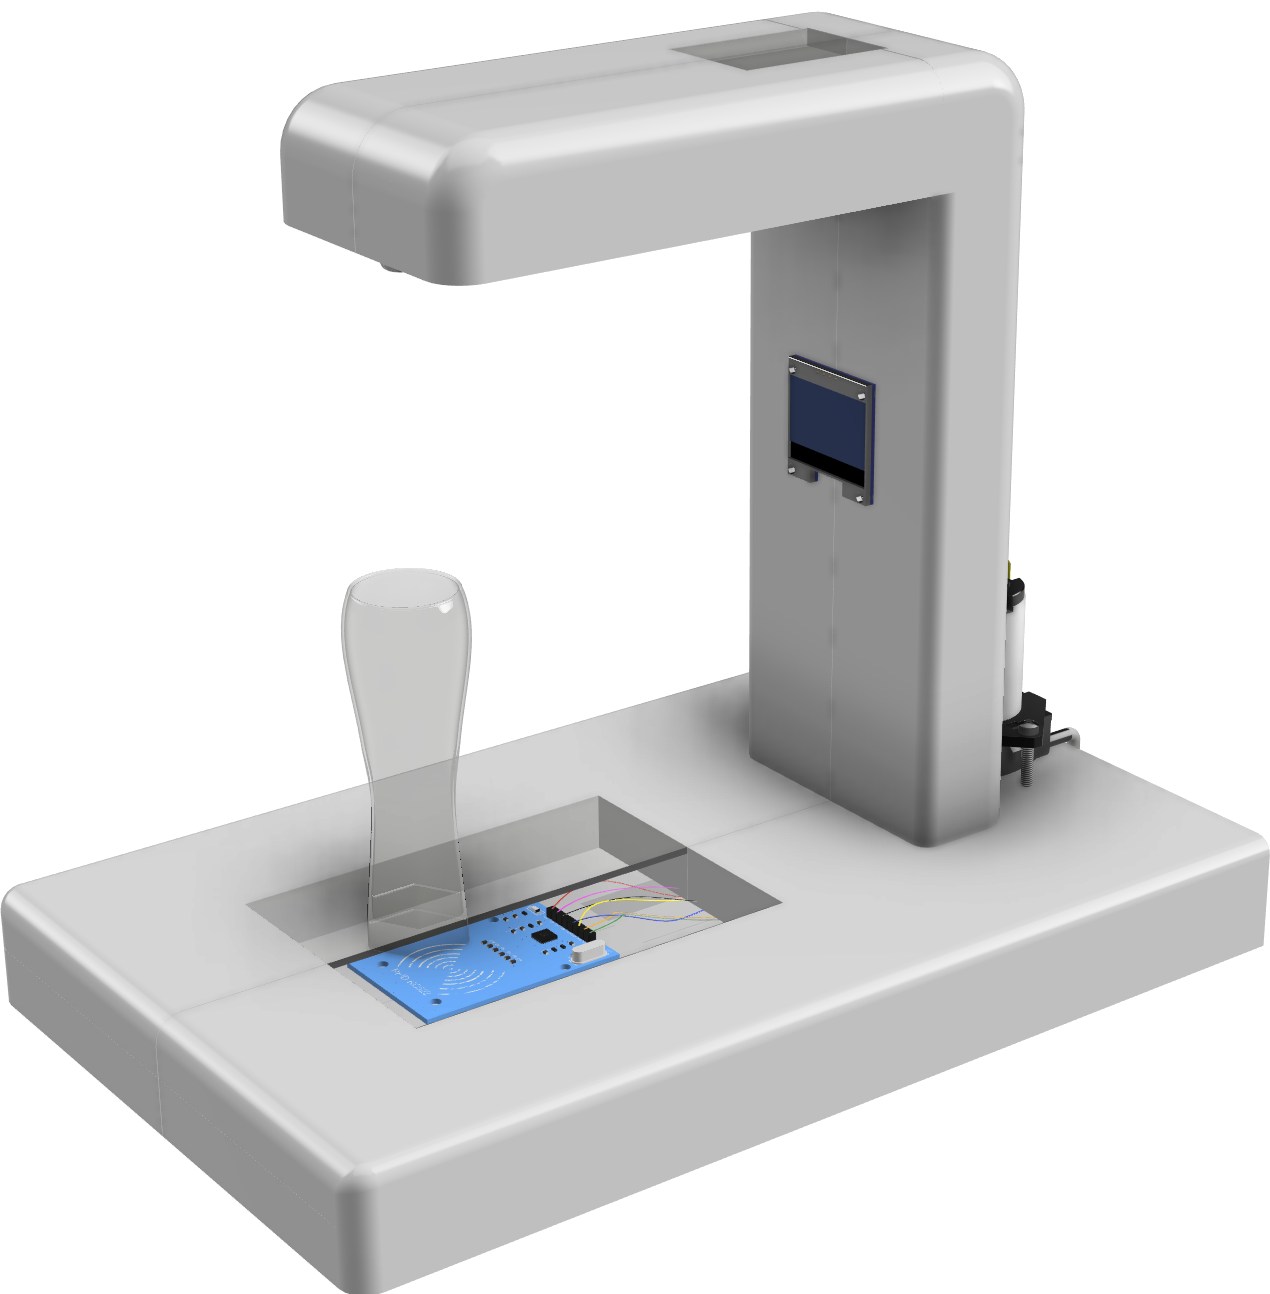
\includegraphics[scale=0.23]{erogatorev13.png}
	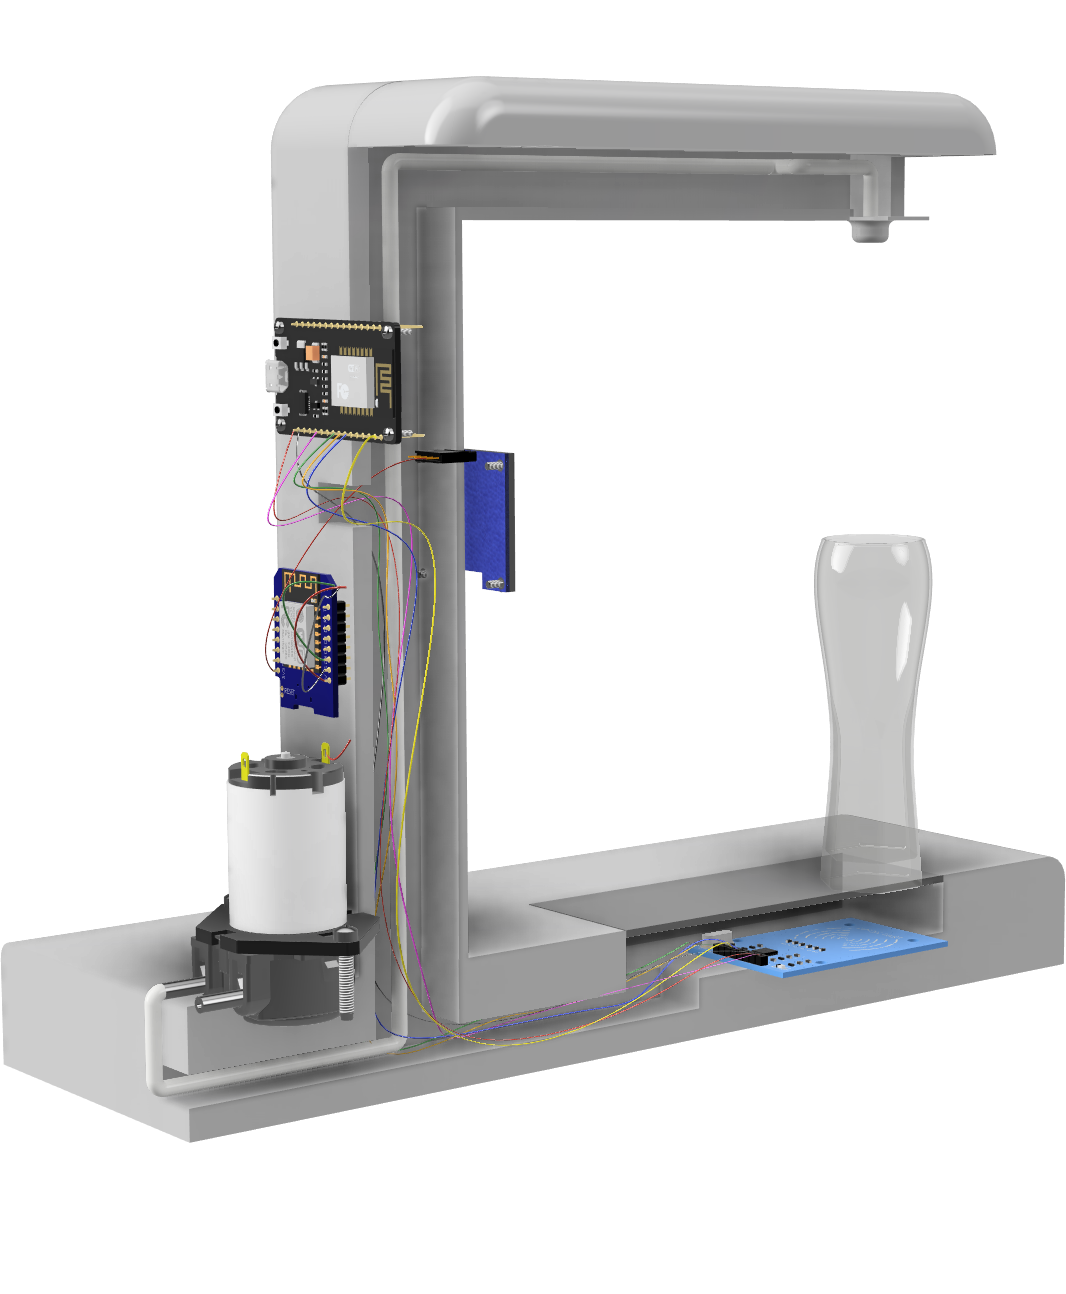
\includegraphics[scale=0.29]{erogatorev12_wires.png}
	\caption{The 3D renders of the refilling station: the first one is a front view, and the other is a section of the station showing the cables and pipes.}
	\label{fig:3dmodelfront1}
\end{figure}


%% Parte conclusiva del documento; tipicamente per riassunto, bibliografia e/o indice analitico.
\backmatter

%% Bibliografia (praticamente obbligatoria)
\bibliographystyle{ieeetr}%% Carica l'omonimo file .bst, dove \languagename � la lingua attiva.
%% Nel caso in cui si usi un file .bib (consigliato)
\bibliography{thud}
%% Nel caso di bibliografia manuale, usare l'environment thebibliography.

%% Per l'indice analitico, usare il pacchetto makeidx (o analogo).

\end{document}

--- Istruzioni per l'aggiunta di nuove lingue ---
Per ogni nuova lingua utilizzata aggiungere nel preambolo il seguente spezzone:
    \addto\captionsitalian{%
        \def\abstractname{Sommario}%
        \def\acknowledgementsname{Ringraziamenti}%
        \def\orcontactsname{Contatti dell'autore}%
        \def\candidatename{Candidato}%
        \def\chairname{Direttore}%
        \def\conclusionsname{Conclusioni}%
        \def\cosupervisorname{Co-relatore}%
        \def\cosupervisorsname{Co-relatori}%
        \def\cyclename{Ciclo}%
        \def\datename{Anno accademico}%
        \def\indexname{Indice analitico}%
        \def\institutecontactsname{Contatti dell'Istituto}%
        \def\introductionname{Introduzione}%
        \def\prefacename{Prefazione}%
        \def\reviewername{Controrelatore}%
        \def\reviewersname{Controrelatori}%
        %% Anno accademico
        \def\shortdatename{A.A.}%
        \def\summaryname{Riassunto}%
        \def\supervisorname{Relatore}%
        \def\supervisorsname{Relatori}%
        \def\thesisname{Tesi di \expandafter\ifcase\csname thud@target\endcsname Laurea\or Laurea Magistrale\or Dottorato\fi}%
        \def\tutorname{Tutor aziendale%
        \def\tutorsname{Tutor aziendali}%
    }
sostituendo a "italian" (nella 1a riga) il nome della lingua e traducendo le varie voci.
